\chapter{Aspectos Teóricos}
\noindent
Este capítulo presenta los prerrequisitos necesarios para obtener los resultados que se encuentran a
lo largo de esta tesis.
En primer lugar, la sección \ref{sec:prerreq} recopila resultados básicos de teoría de números y de
programación lineal. Estas herramientas forman parte de la literatura tradicional y constituyen lo
mínimo necesario para la derivación de nuestros propios resultados.
En segundo lugar, la sección \ref{sec:foundations} presenta enunciados y definiciones obtenidos de
\cite{herr}, los cuales utilizaremos para continuar con la construcción de nuestros propios
resultados que, en pleno conocimiento del autor, son originales.

Como mencionamos en la motivación de esta tesis, nos concentraremos casi exclusivamente en problemas
de programación lineal entera del tipo
\begin{subequations}
	\label{theory:formulation}
	\begin{align}
		\max_{\vec{x} \in \Z^n} \quad
			& \vec{p}^T\vec{x}, \label{theory:objective} \\
		\text{s.a.} \quad
			& \vec{p}^T\vec{x} \leq u, \label{theory:constraint:budget} \\
			& \vec{x} \geq \vec{0}. \nonumber
	\end{align}
\end{subequations}

En la sección \ref{sec:foundations} analizaremos a profundidad este problema, cuyo punto de
culminación será el teorema \ref{theory:th:feasibility}. De manera resumida, el análisis de este
problema se divide en dos casos, dependiendo de los signos de las entradas de un vector $\vec{q}$
asociado a $\vec{p}$.

Observemos que, para este problema, podemos suponer sin pérdida de generalidad que todas las
entradas de $\vec{p}$ son distintas de cero. En efecto, si alguna entrada $p_i$ es cero, podremos
decir que $x_i = 0$. Cuando introduzcamos en el capítulo 4 múltiples restricciones nos desharemos de
este supuesto.

\section{Prerrequisitos}
\label{sec:prerreq}
\noindent
El autor consideró pertinente no incluir demostraciones en esta sección, pues los enunciados son
mostrados en cualquier clase de álgebra superior, programación lineal, o investigación de
operaciones. Las referencias principales para las subsecciones de teoría de números y de
programación lineal son \cite{carmen} y \cite{fabs}, respectivamente.

\subsection{Teoría de Números}
\label{section:number-theory}
\subsubsection{Máximo común divisor y mínimo común múltiplo}
\noindent

\begin{definition}
	Dados dos enteros $a$ y $b$, decimos que \textbf{$a$ divide a $b$} (y escribimos $a \mid b$) si
	existe un entero $k$ tal que $a = k \cdot b$. También denotamos por $D(a)$ al \textbf{conjunto de
	divisores de $a$}, es decir, definimos
	\begin{equation*}
		D(a) \coloneq \braces{b \in \Z \vcentcolon b \mid a}.
	\end{equation*}
\end{definition}
\begin{observation}
	Si $a$ es distinto de cero, entonces $D(a)$ es finito. En efecto, si $b \mid a$ y $a \neq 0$, es
	posible mostrar que $|b| \leq |a|$, lo cual implica que $|D(a)| \leq 2|a|$. En caso de que $a$
	sea nulo, se sigue que $D(a) = \Z$.
\end{observation}
\begin{observation}
	Para cualquier entero $a$ se satisface $\lbrace -1, 1 \rbrace \subseteq D(a)$, pues $a = a \cdot
	1$ y también $a = (-a) \cdot (-1)$.
\end{observation}

\begin{definition}
	\label{prerreq:def:gcd}
	Sean $a_1, \ldots, a_n$ enteros no todos iguales a cero, entonces definimos su \textbf{máximo
	común divisor} $d$ como el elemento maximal del conjunto $\bigcap_{i=1}^{n}D(a_i)$, y escribimos
	$d = \gcd{a_1, \ldots, a_n}$. Si $d = 1$, entonces decimos que $a_1, \ldots, a_n$ son
	\textbf{coprimos}.
\end{definition}

Puesto que alguna entrada $a_i$ es distinta de cero en la definición anterior, encontramos que el conjunto
$\bigcap_{i=1}^{n}D(a_i)$ es finito y también es no vacío (ver observación anterior), por lo que
este conjunto tiene un elemento maximal. Es decir, el máximo común divisor $d$ siempre está bien
definido.
\begin{observation}
	El máximo común divisor siempre es positivo, pues se cumple que $1 \in D(a)$ para todo entero
	$a$, lo que implica por maximalidad que $1 \leq \gcd{a_1, \ldots, a_n}$ para cualquier colección
	de enteros no todos nulos.
\end{observation}

La definición más común del máximo común es dada de manera inductiva. Decimos que $d$ es el máximo
común divisor de dos enteros $a_1, a_2$, no ambos iguales a cero, si se satisface
\begin{enumerate}
	\item $d \mid a_1$ y $d \mid a_2$, y también,
	\item si $d' \mid a_1$ y $d' \mid a_2$, entonces $d' \mid d$.
\end{enumerate}
Luego, para un conjunto de enteros $a_1, a_2 \ldots a_n$, no todos iguales a cero, definimos el máximo común
divisor entre ellos a partir de
\begin{equation*}
	\gcd{a_1, a_2, \ldots, a_{n-1}, a_n} \coloneq \gcd{a_1, \gcd{a_2, \ldots, \gcd{a_{n-1}, a_n}}}.
\end{equation*}
Sin embargo, debemos ser cuidadosos con esta manera de definir las cosas, pues puede ser el caso,
por ejemplo, que $a_{n-1}$ y $a_n$ sean ambos cero y entonces $\gcd{a_{n-1}, a_n}$ no está bien definido.

Para que esta manera de definir el máximo común divisor sea equivalente a la definición
\ref{prerreq:def:gcd}, deberemos presuponer o bien que $a_{n - 1} \neq 0$ o bien que $a_n \neq 0$. A
partir de este punto usaremos ambas definiciones de manera indistinta. Independientemente de qué
definición usemos, la manera de calcular el máximo común divisor siempre es a través del Algoritmo
de Euclides.

\begin{observation}
	No porque una colección de enteros sea coprima se sigue que estos enteros son coprimos a pares.
	Por ejemplo, los enteros 1, 3 y 3 son coprimos pero evidentemente 3 y 3 no lo son.
\end{observation}

\begin{definition}
	Decimos que $c \in \Z$ es una \textbf{combinación lineal entera} de un conjunto de enteros $a_1, \ldots,
	a_n$ si existen enteros $x_1, \ldots, x_n$ tales que $c = a_1x_1 + \cdots + a_nx_n$. Si $c$ es
	positivo, también decimos que esto último es una \textbf{combinación lineal entera positiva}.
\end{definition}

% El siguiente teorema, a pesar de su simpleza, es central para los resultados obtenidos en esta
% tesis.
\begin{theorem}
	\label{prerreq:th:bezout}
	Sea $d$ un entero y sean $a_1, \ldots, a_n$ una colección de enteros no todos iguales a cero.
	Entonces $d = \gcd{a_1, \ldots, a_n}$ si y solo si $d$ es la mínima combinación lineal entera
	positiva de $a_1, \ldots, a_n$.
\end{theorem}

\begin{example}
	El máximo común divisor $d$ de los enteros $a_1 \coloneq 2$, $a_2 \coloneq 3$ y $a_3 \coloneq 5$
	es 1 y además se cumple que $-3a_1 - a_2 + 2a_3 = 1 = d$.
\end{example}

\begin{lemma}
	\label{prerreq:lemma:gcd}
	Si $d = \gcd{a_1, \ldots, a_n}$, entonces $\gcd{\frac{a_1}{d}, \ldots, \frac{a_n}{d}} = 1$.
\end{lemma}

Además del máximo común divisor, haremos uso del mínimo común múltiplo, aunque será en menor medida.
\begin{definition}
	Definimos el \textbf{conjunto de múltiplos} de un entero $a$ como
	\begin{equation*}
		M(a) \coloneq \braces{x \in \Z \vcentcolon a \mid x}.
	\end{equation*}
	También definimos el \textbf{mínimo común múltiplo} de un conjunto de enteros $a_1, \ldots,
	a_n$, no todos iguales a cero, como el elemento minimal del conjunto $\Z_{\geq 0} \cap
	\bigcap_{i=1}^{n}M(a_i)$. Escribimos $\lcm{a_1, \ldots, a_n}$ para denotar a este mínimo común
	múltiplo.
\end{definition}

\begin{observation}
	Si $a$ es nulo, entonces $M(a) = \braces{0}$. En caso contrario encontramos que $M(a)$ es un
	conjunto infinito.
\end{observation}

Para mostrar que el múltiplo común múltiplo está bien definido, basta observar que el producto $|a_1
\cdots a_n|$ es no negativo y también es un elemento de $M(a_i)$ para toda $i \in \braces{1, \ldots,
n}$.

\subsubsection{Ecuaciones lineales diofantinas}

\noindent
Sea $c \in \Z$ y sean $a_1, \ldots, a_n$ enteros. Una ecuación lineal diofantina es una ecuación
donde deseamos determinar enteros $x_1, \ldots, x_n$ que satisfagan
\begin{equation*}
	a_1x_1 + \cdots + a_nx_n = c.
\end{equation*}
Será de nuestro interés en las siguientes secciones resolver iterativamente este tipo de ecuaciones.
Por el momento basta mencionar que podemos enfocarnos en el caso $n = 2$ sin ninguna pérdida de
generalidad. No obstante, los resultados se mantienen para cualquier $n \in \N$.

Los siguientes enunciados abordan el problema de determinar la existencia de soluciones para este
tipo de ecuaciones, así como de construir estas soluciones.
\begin{theorem}[Existencia]
	\label{prerreq:th:existence}
	Sean $a$ y $b$ enteros, no ambos iguales a cero. Entonces la ecuación lineal diofantina $ax + by
	= c$ tiene solución entera si y solo si $\gcd{a, b} \mid c$.
\end{theorem}

Para construir el conjunto de soluciones a una ecuación lineal diofantina, primero encontramos  una
solución particular.
\begin{definition}
	\label{prerreq:def:bezout}
	Sea $d \coloneq \gcd{a, b}$ y sean $x', y'$ enteros tales que $ax' + by' = d$ (c.f. teorema
	\ref{prerreq:th:bezout}). Decimos entonces que $x', y'$ son \textbf{coeficientes de Bézout} asociados a
	$a$ y $b$, respectivamente\footnote{
		Los coeficientes de Bézout se pueden calcular a través del Algoritmo Extendido de Euclides.
		Véase \url{https://en.wikipedia.org/wiki/Extended_Euclidean_algorithm}.
	}.
\end{definition}

\begin{observation}
	Los coeficientes de Bézout asociados a un par de enteros no son únicos. En efecto, si $x', y'$
	son coeficientes de Bézout de $a$ y $b$, entonces $x' + b$, $y' - a$ también lo son:
	\begin{equation*}
		a(x' + b) + b(y' - a) = ax' + by' + ab - ab = ax' + by' = d.
	\end{equation*}
	Para fines de esta tesis basta la existencia de estos coeficientes, por lo que decimos de manera
	indistinta ``los coeficientes de Bézout'' y ``una elección de coeficientes de Bézout''.
\end{observation}

Definamos $d \coloneq \gcd{a, b}$ y supongamos que la ecuación $ax + by = c$ tiene solución.
Por el teorema \ref{prerreq:th:existence}, se sigue que $d \mid c$, y entonces existe $c' \in \Z$
tal que $c = c' \cdot d$. Sean $x', y'$ los coeficientes de Bézout asociados a $a, b$
respectivamente. Así,
\begin{equation*}
	a(c' \cdot x') + b(c' \cdot y') = c'(ax' + by') = c'd = c,
\end{equation*}
por lo que $(c' \cdot x', c' \cdot y')$ es una solución particular de la ecuación $ax + by = c$.

\begin{theorem}[Construcción]
	\label{prerreq:th:construction}
	Sea $(x_0, y_0)$ una solución particular de la ecuación lineal diofantina $ax + by = c$.
	Entonces todas las soluciones enteras de aquella ecuación están dadas por
	\begin{equation}
		\label{prerreq:eq:construction}
		\begin{cases}
			x = x_0 + \frac{b}{d}t, \\
			y = y_0 - \frac{a}{d}t,
		\end{cases}
	\end{equation}
	donde $d \coloneq \gcd{a, b}$ y $t \in \Z$ es una variable libre.
\end{theorem}

\begin{example}
	Consideremos la ecuación lineal $2x + 3y = 5$. Los coeficientes de Bézout asociados a 2 y 3 son,
	respectivamente, -1 y 1. Luego, una solución particular para la ecuación es $(x_0, y_0) = (-5, 5)$.
	Por el teorema anterior encontramos que todas las soluciones están dadas por
	\begin{equation*}
		\begin{cases}
			x = -5 + 3t, \\
			y = 5 - 2t,
		\end{cases}
	\end{equation*}
	donde $t \in \Z$ es una variable libre. En efecto, sustituyendo obtenemos
	\begin{equation*}
		2(-5 + 3t) + 3(5 - 2t) = -10 + 15 + 6t - 6t = 5.
	\end{equation*}
\end{example}

\subsection{Programación lineal}
\label{subsec:lp}
\noindent
La programación lineal se encarga de resolver problemas de optimización de la forma
\begin{equation}
	\label{prim:lineal-opt}
	\max_{\vec{x}} ~\lbrace \vec{c}^T\vec{x} \colon \vec{x} \in P \rbrace,
\end{equation}
donde $P$ es un poliedro.

En esta sección repasamos brevemente propiedades del poliedro $P$ al cual llamamos región factible.
Así también, indicamos dónde se encuentra el óptimo del problema \eqref{prim:lineal-opt} y hacemos
mención rápida sobre cómo obtenerlo. Finalmente, nos enfocamos en programas lineales enteros y, más
importantemente, describimos cómo funciona el algoritmo de Ramificación y Acotamiento para encontrar
soluciones de estos programas enteros.

\begin{definition}
	Sea $\vec{a} \in \R^n$ un vector no nulo y sea $b \in \R$ un escalar. Llamamos
	\textbf{hiperplano afino}
	al conjunto de vectores $\vec{x} \in \R^n$ que satisfacen $\vec{a}^T\vec{x} = b$. Así también,
	llamamos \textbf{semi-espacios afinos} a los conjuntos de vectores $\vec{x}, \vec{y} \in \R^n$ que
	satisfacen $\vec{a}^T\vec{x} \geq b$ y $\vec{a}^T\vec{y} \leq b$.
\end{definition}

\begin{definition}
	Sea $A \in \R^{m \times n}$ una matriz con renglones linealmente independientes y $\vec{b} \in
	\R^m$ un vector. Entonces al conjunto definido por
	\begin{equation}
		\label{prerreq:def:poly}
		P \coloneq \lbrace \vec{x} \in \R^n \colon A\vec{x} \geq \vec{b} \rbrace
	\end{equation}
	lo llamamos \textbf{poliedro}. Si, además, $P$ es acotado, entonces decimos que $P$ es un
	\textbf{politopo}.
\end{definition}

\begin{observation}
	Todo poliedro $P$ definido de esta manera representa la intersección de $m$ semi-espacios
	afinos. Esto se debe a que $A\vec{x} \geq \vec{b}$ si y solo si $\vec{a}_i^T\vec{x} \geq b_i$
	para toda $1 \leq i \leq m$ y donde $\vec{a}_i^T$ representa el $i$-ésimo renglón de la matriz
	$A$. En la Figura \ref{fig:hyp} se muestra visualmente esta relación entre hiperplanos afinos y
	poliedros.
\end{observation}

\begin{figure}[ht]
	\centering
	\begin{minipage}{0.45\textwidth}
		\centering
		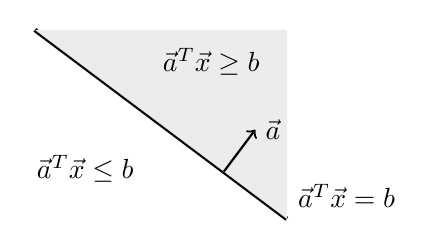
\begin{tikzpicture}[scale=0.8]
			% hyperplane
			\draw[ultra thick, black] (-2,1) -- (2,-2) node[above right] {$\vec{a}^T\vec{x} = b$};
			% labels
			\node at (-1.2,-1.2) {${\vec{a}^T \vec{x} \leq b}$};
			%shading
			\fill[gray!15, domain=-2:2, variable=\x]
				(-2,1) -- plot ({\x}, {-0.75*\x - 0.5}) -- (2,1) -- cycle;
			\draw[->, thick] (1,-1.25) -- (1.5,-0.583) node[right] {$\vec{a}$};
			\node at (0.8,0.5) {${\vec{a}^T \vec{x} \geq b}$};
		\end{tikzpicture}
	\end{minipage}
	\begin{minipage}{0.45\textwidth}
		\centering
		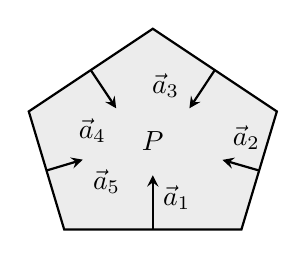
\begin{tikzpicture}[scale=1.5, >=stealth]
			% coordinates
			\coordinate (A) at (0,0);
			\coordinate (B) at (1.5,0);
			\coordinate (C) at (1.8,1);
			\coordinate (D) at (0.75,1.7);
			\coordinate (E) at (-0.3,1);
			% pentagon
			\filldraw[fill=gray!15, thick]
			(A) -- (B) -- (C) -- (D) -- (E) -- cycle;
		  % normal vectors
			% AB
			\draw[->, black, thick] (0.75,0) -- (0.75,0.46) node[below right] {$\vec{a}_1$};
			% BC
			\draw[->, black, thick] (1.65,0.5) -- (1.34,0.59) node[above right] {$\vec{a}_2$};
			% CD
			\draw[->, black, thick] (1.275,1.35) -- (1.06,1.027) node[above left] {$\vec{a}_3$};
			% DE
			\draw[->, black, thick] (0.225,1.35) -- (0.44,1.027) node[below left] {$\vec{a}_4$};
			% EA
			\draw[->, black, thick] (-0.15,0.5) -- (0.157,0.592) node[below right] {$\vec{a}_5$};
			% polyhedron label
			\node at (0.75, 0.75) {$P$};
		\end{tikzpicture}
	\end{minipage}
	\caption{\textit{Izquierda:} Un hiperplano afino $\braces{\vec{x} \colon \vec{a}^T\vec{x} = b}$
	junto con los dos semi-espacios que induce. \textit{Derecha:} Un politopo $P$.}
	\label{fig:hyp}
\end{figure}

\begin{definition}
	Sea $P$ un poliedro. Decimos que el vector $\vec{x} \in P$ es un \textbf{vértice} de $P$ si existe
	$\vec{c} \in \R^n$ de manera que $\vec{c}^T\vec{x} < \vec{c}^T\vec{y}$ para todo $\vec{y} \in P
	\setminus \braces{\vec{x}}$.
\end{definition}

En términos gráficos, decimos que $\vec{x}$ es un vértice si se satisfacen dos condiciones: en
primer lugar, existe un hiperplano afino que pasa por $\vec{x}$ y uno de sus semi-espacios inducidos
contiene completamente al poliedro $P$; en segundo lugar, ningún otro punto de $P$ se encuentra
sobre este hiperplano.

\begin{definition}
Sea $P$ un poliedro y sea $\vec{c} \in \R^n$ un vector. Todo problema de optimización de la forma
\eqref{prim:lineal-opt} entra en una de las siguientes tres categorías:
\begin{enumerate}
	\item El valor óptimo no existe: ningún vector $\vec{x} \in \R^n$ satisface
		el sistema de desigualdades $A\vec{x} \geq \vec{b}$. Es decir, la región factible es vacía.
	\item El valor óptimo existe y es infinito: el poliedro $P$ no es acotado y
		somos capaces de encontrar una sucesión de vectores $\lbrace \vec{x}_k \rbrace_{k \in \N}$
		en el poliedro $P$ que satisface $\vec{c}^T\vec{x}_{k+1} > \vec{c}^T\vec{x}_k$ para todo $k \in \N$.
	\item El valor óptimo existe y es finito: este caso es la negación de los dos casos anteriores,
		pero cabe recalcar que esto no significa que el poliedro $P$ es acotado.
\end{enumerate}
En el primer caso decimos que \textbf{el problema es infactible}, mientras que en los últimos dos
decimos que \textbf{el problema es factible}. También diremos comúnmente del segundo caso que
\textbf{el problema es no acotado}.
\end{definition}

Es posible mostrar que todo poliedro $P \coloneq \lbrace \vec{x} \in \R^n \colon A\vec{x} \geq
\vec{b} \rbrace$ puede ser transformado a la forma estándar
\begin{equation*}
	\lbrace \left( \vec{x}^+, \vec{x}^-, \vec{s} \right) \in \R^{n + n + m} \colon A(\vec{x}^+ -
\vec{x}^-) - \vec{s} = \vec{b}, \left(\vec{x}^+, \vec{x}^-, \vec{s}\right) \geq \vec{0}\rbrace,
\end{equation*}
de manera que todo problema de optimización de la forma \eqref{prim:lineal-opt} puede ser escrito
sin pérdida de generalidad como
\begin{subequations}
	\label{prerreq:formulation}
	\begin{align}
		\max_{\vec{x} \in \R^n} \quad
			& \vec{c}^T\vec{x}, \label{prerreq:formulation:objective} \\
		\text{s.a.} \quad
			& A\vec{x} = \vec{b}, \label{prerreq:formulation:constraints} \\
			& \vec{x} \geq \vec{0} \nonumber.
	\end{align}
\end{subequations}
De ahora en adelante nuestro análisis se concentrará exclusivamente en problemas lineales de este
tipo. Es decir, supondremos, sin pérdida de generalidad, que todo problema lineal se encuentra en
esta forma estándar.

\begin{theorem}
	\label{prerreq:th:linear-sol}
	Sea $P$ un poliedro que tiene al menos un vértice, consideremos el problema
	\eqref{prerreq:formulation}, y supongamos que el valor óptimo $z^*$ existe y es finito. Entonces
	el conjunto de soluciones óptimas contiene al menos un vértice de $P$.
\end{theorem}

Este teorema fundamental constituye el primer paso para la construcción de varios algoritmos que
encuentran soluciones del problema \eqref{prerreq:formulation}. Ciertamente, el más famoso de todos
es el algoritmo simplex, el cual ``salta'' de vértice en vértice hasta llegar a uno con valor
óptimo. Otros, más modernos y conocidos como métodos de puntos interiores, comienzan en el interior
del poliedro $P$ y son ``atraídos'' como imanes a uno de los vértices con valor óptimo. No es el
objetivo de esta tesis exponer la maquinaria matemática detrás de estos algoritmos\footnote{
	Sin embargo, la literatura para explicar estos métodos es abundante. Véase, por ejemplo,
	\cite{nocedal}.
}.

Ahora describimos brevemente los programas lineales enteros y pasamos a explicar el método de
Ramificación y Acotamiento. Por ello, lo que se encuentra a continuación supone que contamos con un
algoritmo para resolver problemas del tipo \eqref{prerreq:formulation}.
\begin{definition}
	Sea $A \in \R^{m \times n}$ una matriz con renglones linealmente independientes y sea $\vec{b}
	\in \R^m$ un vector. Al problema de optimización lineal \eqref{prerreq:formulation} lo llamamos
	\textbf{problema relajado} del programa lineal entero
	\begin{subequations}
		\label{prerreq:formulation:ilp}
		\begin{align}
			\max_{\vec{x} \in \Z^n} \quad
				& \vec{c}^T\vec{x}, \label{prerreq:formulation:objective:ilp} \\
			\text{s.a.} \quad
				& A\vec{x} = \vec{b}, \label{prerreq:formulation:constraints:ilp} \\
				& \vec{x} \geq \vec{0} \nonumber.
		\end{align}
	\end{subequations}
\end{definition}
Resalta el hecho de que la formulación de un programa lineal entero es idéntico a su formulación
relajada, solamente agregamos la restricción de que nuestra solución óptima $\vec{x}^*$
sea entera. Es decir, lo único que cambia es la región de factibilidad. De hecho, si
definimos el poliedro
\begin{equation*}
	P \coloneq \lbrace \vec{x} \in \R^n \colon A\vec{x} = \vec{b}, \vec{x} \geq \vec{0} \rbrace,
\end{equation*}
entonces tenemos que $P \cap \Z^n$ corresponde a la región factible de
\eqref{prerreq:formulation:ilp}, mientras que $P$ corresponde a la región factible de su problema
relajado.

A partir de lo anterior, deducimos inmediatamente que el valor óptimo $\optilp{z}$ de un programa
entero es una cota inferior del valor óptimo $z^*$ de su problema relajado, pues ambos son problemas
de maximización y es cierto que $P \cap \Z^n \subseteq P$. De aquí se sigue que si $\optilp{z} =
z^*$, entonces la solución óptima $\vec{x}^*$ del problema relajado también es la solución
óptima del programa lineal entero si $\vec{x}^* \in \Z^n$.

El algoritmo estándar para encontrar soluciones de programas lineales enteros es Ramificación y
Acotamiento. Este método consiste en generar un árbol binario donde cada nodo representa un
subproblema lineal a resolver. En la raíz del árbol resolvemos el problema relajado
\eqref{prerreq:formulation} y, si la solución óptima $\vec{x}^* \in \R^n$ no es entera, entonces
para alguna entrada $x_i^*$ no entera agregamos la restricción $x_i \leq \lfloor x_i^* \rfloor$ para
crear un subproblema, y también añadimos la restricción $x_i \geq \lceil x_i^* \rceil$ para crear
otro subproblema. Este procedimiento se realiza de manera recursiva.

Observemos que, si decidimos recorrer todos los nodos del árbol binario, entonces tendremos que
resolver al menos $2^n$ subproblemas, donde $n$ es la dimensión del problema lineal. Por esta razón,
el algoritmo cuenta con políticas para deshacerse de subárboles que nunca proveerán la solución
óptima. El autor considera que es mejor ilustrar estas políticas a partir de un ejemplo. El
Algoritmo \ref{algo:bb} en el Apéndice \ref{app:bb} presenta una versión rudimentaria del método de
Ramificación y Acotamiento.

\begin{example}[\cite{fabs}]
	\label{ex:ilp}
	Consideremos el programa lineal entero
	\begin{align*}
		\max_{\vec{x} \in \Z^2} \quad
			& 4x_1 - x_2, \\
			\text{s.a.} \quad
			& 7x_1 - 2x_2 \leq 14, \\
			& 2x_1 - 2x_2 \leq 3, \\
			& x_2 \leq 3, \\
			& x_1, x_2 \geq 0.
	\end{align*}
	La región factible de este problema se muestra en la Figura \ref{fig:feas}. La solución al problema
	relajado, cuya región factible denotamos por $S_0$, está dada por $\vec{x}^0 \coloneq (20/7,
	3)^T$. Como $x_1^0 = 20/7$ no es entero, generamos dos nuevos subproblemas con regiones
	factibles
	\begin{align*}
		S_{00} &\coloneq S_0 \cup \braces{ x_1 \leq \floor{20/7} = 2}, \\
		S_{01} &\coloneq S_0 \cup \braces{ x_1 \geq \ceil{20/7} = 3}.
	\end{align*}
	De la Figura \ref{fig:feas}, observamos que $S_{01}$ es vacío y por lo tanto de este problema no
	podemos generar otros subproblemas. En este caso, decimos que \textbf{podamos $S_{01}$ por
	infactibilidad}.

	Ahora bien, la solución al problema $S_{00}$ está dada por $\vec{x}^1 \coloneq (2, 1/2)^T$.
	Encontramos que $x_2^1$ = 1/2 no es entero y por lo tanto generamos dos nuevos subproblemas:
	\begin{align*}
		S_{000} &\coloneq S_{00} \cup \braces{ x_2 \leq \floor{1/2} = 0}, \\
		S_{001} &\coloneq S_{00} \cup \braces{ x_2 \geq \ceil{1/2} = 1}.
	\end{align*}
	Observemos que la solución $\vec{x}^2$ de $S_{001}$ es $(2, 1)^T$, la cual es entera y tiene valor
	objetivo $z_2^* \coloneq 7$. No generamos otros subproblemas a partir de este problema porque
	sus regiones factibles estarán contenidas en $S_{001}$ y por lo tanto sus valores objetivos
	serán menores o iguales al de $S_{001}$. Así pues, decimos que \textbf{podamos $S_{001}$ por
	integralidad}.

	La solución de $S_{000}$, en cambio, es $\vec{x}^3 \coloneq (3/2, 0)^T$ y tendríamos que ramificar
	de nuevo en otros dos subproblemas. No obstante, observemos que el valor objetivo de este
	subproblema es $z_3^* \coloneq 6$, el cual es menor que $z_2^* = 7$. Como la región factible de
	cualquier subproblema generado a partir de este último problema estára contenido en $S_{000}$,
	se sigue que su valor objetivo será menor o igual al de $S_{000}$. Es decir, no encontraremos
	otro vector cuyo valor objetivo sea mayor que $z_2^*$. Decimos entonces que
	\textbf{podamos $S_{000}$ por cota}.

	Como hemos agotado todos los subproblemas que podríamos generar, entonces concluimos que la
	solución óptima de este programa  lineal entero es $\vec{x}^2 = (2, 1)^T$ y tiene valor objetivo
	$z_2^* = 7$.
\end{example}
\begin{figure}
	\centering
	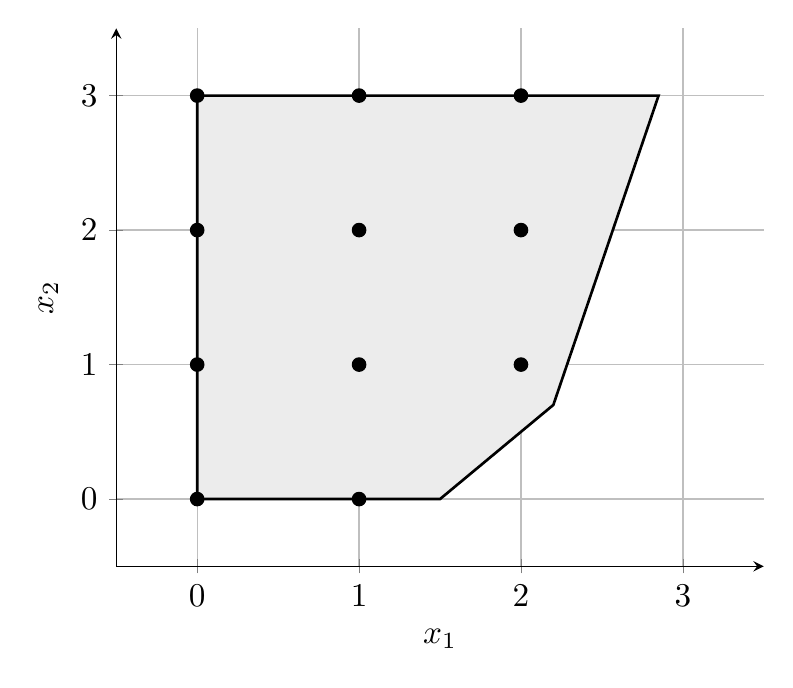
\begin{tikzpicture}[scale=1.2]
		\begin{axis}[
			axis lines=left,
			xmin=-0.5, xmax=3.5,
			ymin=-0.5, ymax=3.5,
			grid=both,
			xlabel=$x_1$,
			ylabel=$x_2$
			]
			\addplot+ [thick,color=black,fill=gray!15,mark=none] table {
				0 0
				1.5 0
				2.2 0.7
				2.85 3
				0 3
				0 3
				0 0
			};
			\addplot+ [only marks,,mark=*,mark options={scale=1, color=black, fill=black}] table {
				0 0
				0 1
				0 2
				0 3
				1 0
				1 1
				1 2
				1 3
				2 1
				2 2
				2 3
			};
		\end{axis}
	\end{tikzpicture}
	\caption{Los puntos negros forman la región factible del programa lineal entero del Ejemplo
	\ref{ex:ilp}, mientras que la región sombreada es la región factible de su problema relajado.}
	\label{fig:feas}
\end{figure}

\section{Fundamentos}
\label{sec:foundations}
\noindent
Esta sección se divide en cuatro partes. En primer lugar, damos a conocer las definiciones y
encunciados provistos por \cite{herr}. Es importante aclarar que el autor tradujo libremente algunos
términos a falta de encontrar fuentes en español que hicieran uso de ellos. En particular, el autor
decidió nombrar ``vectores esencialmente enteros'' a los \textit{projectively rational vectors} (ver
definición \ref{theory:def:rational}) y ``capas enteras'' a los \textit{c-layers} (ver definición
\ref{phase-1:def:c-layer}).

En segundo lugar, mostramos la equivalencia entre resolver problemas del tipo
\eqref{theory:formulation} y resolver ecuaciones lineales diofantinas. Nos basamos en los teoremas
\ref{prerreq:th:existence} y \ref{prerreq:th:construction} para construir inductivamente el conjunto
de soluciones de una ecuación lineal diofantina en $n$ incógnitas. Las soluciones de estas
ecuaciones serán definidas a partir de una relación de recurrencia y también dependerán de una
colección de $n - 1$ parámetros libres.

En tercer lugar, establecemos una transformación lineal entre el conjunto de soluciones de una ecuación
lineal diofantina en $n$ incógnitas y el conjunto de $n - 1$ parámetros libres que determinan estas
soluciones. Luego, investigamos las propiedades de esta transformación lineal que serán de gran utilidad
teórica para los siguientes capítulos, en especial para el capítulo 4.

Finalmente, mostramos que el vector objetivo $\vec{p}$ del problema original
\eqref{theory:formulation} induce una descomposición interesante de $\Z^n$ y analizamos cómo se
relacionan estas descomposiciones al considerar distintos vectores $\vec{p}$. Esto nos permitirá
mostrar equivalencias entre distintas instancias del problema \eqref{theory:formulation}.

\subsection{Capas enteras}
\label{subsec:sym}

\begin{definition}
	\label{theory:def:rational}
	Decimos que un vector $\vec{v} \in \R^n \setminus \lbrace \vec{0} \rbrace$ es
	\textbf{esencialmente entero} si existen un vector $\vec{w} \in \Z^n$ y un escalar $m \neq 0$
	tales que $\vec{v} = m\vec{w}$. Además, decimos que $\vec{w}$ es el \textbf{múltiplo coprimo} de
	$\vec{v}$ si sus entradas son coprimas y si su primera entrada no nula es positiva.
\end{definition}
\begin{example}
	El vector $\left(-\sqrt{2}, 1/\sqrt{2}\right)^T = 2\sqrt{2}(-2, 1)^T$ es esencialmente entero
	y $(2, -1)^T$ es su múltiplo coprimo. En contraste, el vector $\paren{\sqrt{2}, \sqrt{3}}^T$ no es
	esencialmente entero.
\end{example}
\begin{observation}
	Todo vector racional $\vec{v} \in \Q^n \setminus \braces{\vec{0}} $  es esencialmente
	entero. En efecto, para cada $i \in \braces{1, \ldots, n}$ existen $p_i, q_i \in
	\Z$ con $q_i \neq 0$ tales que $v_i = p_i/q_i$. Luego, si definimos $m \coloneq \lcm{q_1,
	\ldots, q_n} \neq 0$ y también $\vec{w} \coloneq m\vec{v} \in \Z^n$, encontramos que $\vec{v} =
	\frac{1}{m}\vec{w}$.
\end{observation}
\begin{observation}
	\label{obs:coprime-unique}
	Todo vector $\vec{v}$ esencialmente entero tiene a lo más dos vectores coprimos asociados. Sean
	$m \in \R$ y $\vec{w} \in \Z^n$ tales que $\vec{v} = m\vec{w}$. Entonces
	\begin{equation*}
		\pm \frac{1}{\gcd{w_1, \ldots, w_n}}\vec{w}
	\end{equation*}
	son dos vectores cuyas entradas son coprimas, de acuerdo al lema \ref{prerreq:lemma:gcd}. Como
	la primera entrada no nula $w_i$ también debe ser positiva, se sigue que solo uno de estos dos
	vectores es el múltiplo coprimo de $\vec{v}$. Así, el múltiplo coprimo de un vector
	esencialmente entero es único.
\end{observation}

Puesto que todo número representable en cualquier sistema de aritmética finita es necesariamente
racional, decidimos enfocar nuestro análisis en vectores esencialmente enteros. Desde el punto de
vista puramente teórico, esta condición reduce de manera drástica el tipo de programas lineales que
podemos resolver. No obstante, esta clase de vectores es un poco más general que los considerados en
otros textos de programación lineal. Por ejemplo, \cite{martello} y \cite{alex} toman en cuenta
vectores puramente racionales.

\begin{definition}
	\label{phase-1:def:c-layer}
	Sea $\vec{v} \in \R^n$ un vector esencialmente entero y sea $t \in \R$ un escalar. Decimos que
	su hiperplano afino asociado
	\begin{equation}
		\label{phase-1:def:affine-hyperplane}
		\clayer{\vec{v}}{t} \coloneq \ker{\vec{x} \mapsto \vec{v}^T\vec{x}} + t\vec{v}
		= \lbrace \vec{v}^{\perp} + t\vec{v} \vcentcolon \vec{v}^T\vec{v}^{\perp} = 0 \rbrace
	\end{equation}
	es una \textbf{capa entera} si contiene al menos un punto entero.
\end{definition}

\begin{lemma}
	\label{phase-1:lemma:layer}
	Sean $\vec{v}, \vec{x} \in \R^n$ con $\vec{v}$ distinto de cero. Entonces $\vec{x} \in
	\clayer{\vec{v}}{t_{\vec{x}}}$, donde $t_{\vec{x}} \coloneq
	\frac{\vec{v}^T\vec{x}}{\norm{\vec{v}}^2}$.
\end{lemma}

Las capas enteras son invariantes ante reescalamientos en el vector $\vec{v}$: si $r \neq 0$,
entonces $\clayer{\vec{v}}{t} = \clayer{r\vec{v}}{t/r}$. En efecto, sea $\vec{x} \in
\clayer{\vec{v}}{t}$. Luego, existe $\vec{v}^\perp$ ortogonal a $\vec{v}$ tal que
\begin{equation*}
	\vec{x} = \vec{v}^\perp + t\vec{v} = \vec{v}^\perp + \frac{t}{r}(r\vec{v}).
\end{equation*}
Pero si $\vec{v}^\perp$ es ortogonal a $\vec{v}$, entonces también es ortogonal a $r\vec{v}$.
Así, encontramos que $\vec{x} \in \clayer{r\vec{v}}{t/r}$. La otra contención se muestra de
manera similar.

En particular, si $\vec{w}$ es el múltiplo coprimo de $\vec{v}$, se cumple que
\begin{equation}
	\label{eq:clayer-eq}
	\braces{\clayer{\vec{v}}{t} \vcentcolon t \in \R}
	=
	\braces{\clayer{\vec{v}/m}{t m} \vcentcolon t \in \R}
	=
	\braces{\clayer{\vec{w}}{t} \vcentcolon t \in \R},
\end{equation}
donde $m \neq 0$ es el escalar que satisface $\vec{v} = m\vec{w}$. Así pues, para analizar las capas
enteras, basta con fijarnos en los múltiplos coprimos que las definen en vez de sus vectores
esencialmente enteros asociados.

\begin{theorem}
	\label{phase-1:th:cover}
	Sea $\vec{v} \in \R^n$ un vector esencialmente entero y sea $\vec{w}$ su múltiplo coprimo.
	Entonces la familia de capas enteras $\braces{\qlayer{w}{k} \vcentcolon k \in \Z}$ cubre a
	$\Z^n$.
\end{theorem}

\begin{lemma}
	\label{theory:lemma:utility}
	Sea $\vec{v} \in \R^n$ un vector esencialmente entero y sea $\vec{w}$ su múltiplo coprimo.
	Entonces $\vec{q}^T\vec{x} = k$ para todo $\vec{x} \in \qlayer{w}{k}$.
\end{lemma}
\begin{proof}
	Sea $\vec{x} \in \qlayer{w}{k}$, por lo que existe un vector $\vec{w}^\perp$ ortogonal a
	$\vec{w}$ tal que
	\begin{equation*}
		\vec{x} = \vec{w}^\perp + \frac{k}{\norm{\vec{w}}^2}\vec{w}.
	\end{equation*}
	Luego,
	\begin{equation*}
		\vec{w}^T\vec{x} = \vec{w}^T\vec{w}^\perp + \frac{k}{\norm{\vec{w}}^2}\vec{w}^T\vec{w}
		=
		0 + \frac{k}{\norm{\vec{w}}^2}\norm{\vec{w}}^2 = k.
	\end{equation*}
	que es lo que deseábamos obtener.
\end{proof}

% Pasemos a considerar el programa lineal (\ref{theory:formulation}) donde $\vec{p}$ es un vector
% esencialmente entero y $\vec{q}$ es su múltiplo coprimo. Comúnmente a la función objetivo
% (\ref{theory:objective}) le daremos el nombre de utilidad y a la restricción
% (\ref{theory:constraint:budget}) la llamaremos restricción presupuestaria, así como presupuesto al
% lado derecho de esta restricción.

Consideremos el problema \eqref{theory:formulation} y supongamos que el vector objetivo $\vec{p}$ es
esencialmente entero. Sea $\vec{q}$ su múltiplo coprimo. Sabemos de \eqref{eq:clayer-eq} que 
	$\braces{\clayer{\vec{p}}{t} \vcentcolon t \in \R}
	=
	\braces{\clayer{\vec{q}}{t} \vcentcolon t \in \R}$.
Puesto que nos concentramos en puntos enteros, por el teorema \ref{phase-1:th:cover} podemos
considerar exclusivamente el subconjunto de capas enteras $\braces{\qlayer{q}{k} \vcentcolon k \in
\Z}$.

Observemos del lema \ref{theory:lemma:utility} junto con la restricción presupuestaria
\eqref{theory:constraint:budget} que los puntos enteros de la \textbf{$k$-ésima capa entera}
$\qlayer{q}{k}$ o bien respetan todos esta restricción o bien ninguno la respeta. Nos gustaría
entonces determinar el primer parámetro $\eta \in \Z$ que induce a que todos los puntos enteros de
$\qlayer{q}{\eta}$ respeten la restricción presupuestaria.

Para respetar la restricción \eqref{theory:constraint:budget}, debe ser el caso que
todo $\vec{x} \in \qlayer{q}{k}$ satisfaga
\begin{equation}
	\label{eq:eta-cases}
	\vec{p}^T\vec{x} = m\vec{q}^T\vec{x} = mk \leq u
	\iff
	\begin{cases}
		k \geq u/m, & m < 0, \\
		k \leq u/m, & m > 0,
	\end{cases}
\end{equation}
donde $m \neq 0$ es el escalar que satisface $\vec{p} = m\vec{q}$. Así pues, dependiendo del signo
de $m$, tenemos que el primer parámetro $\eta$ en satisfacer la restricción presupuestaria puede ser
interpretado como el entero más pequeño o el entero más grande que satisface su respectiva
desigualdad.

\begin{lemma}
	\label{phase-1:lemma:eta}
	Sea $\vec{p} \in \R^n$ un vector esencialmente entero y sea $\vec{q}$ su múltiplo coprimo, de
	manera que $\vec{p} = m\vec{q}$ para algún escalar $m \neq 0$. Entonces la primera capa entera
	$\qlayer{q}{\eta}$ que satisfacen la restricción \eqref{theory:constraint:budget} está
	parametrizada por
	\begin{equation}
		\label{lemma:eq:eta-cases}
		\eta \coloneq \begin{cases}
			\ceil{u/m}, & m < 0, \\
			\floor{u/m}, & m > 0.
		\end{cases}
	\end{equation}
\end{lemma}
\begin{proof}
	Se sigue inmediatamente de \eqref{eq:eta-cases}.
\end{proof}

Puesto que la gran mayoría de nuestros enunciados y algoritmos dependen de este primer parámetro
$\eta$, tendremos que separarlos al menos en dos casos. Por ello, el autor creyó prudente
considerar solamente el caso $m > 0$, aunque cabe mencionar que los enunciados y demostraciones para
el caso $m < 0$ son completamente análogos, donde las diferencias recaen en que el orden de las
desigualdades cambian o las funciones piso se reemplazan por funciones techo, por ejemplo.

En resumen, si $m > 0$, encontramos que las capas enteras que satsifacen la restricción
\eqref{theory:constraint:budget} están parametrizadas por $k \in \braces{\eta, \eta - 1, \ldots}$,
donde $\eta$ está definida en \ref{phase-1:lemma:eta}. Además, por el lema
\ref{theory:lemma:utility}, todo $\vec{x} \in \qlayer{q}{k}$ satisface la ecuación $\vec{q}^T\vec{x} = k$.
\begin{theorem}
	\label{theory:th:infeasibility}
	Sea $\vec{p} \in \R^n$ un vector esencialmente entero y sea $\vec{q}$ su múltiplo coprimo.
	Entonces el problema \eqref{theory:formulation} es infactible si y solo si $\vec{q} \geq
	\vec{0}$ y el lado derecho $u$ de \eqref{theory:constraint:budget} es negativo. 
\end{theorem}
\begin{proof}
	Supongamos que $\vec{q} \geq \vec{0}$ y $u < 0$. Si $\vec{x} \in \Z_{\geq \vec{0}}^n$
	entonces $\vec{q}^T\vec{x} \geq 0 > u$ y por lo tanto $\vec{x}$ no es factible. Luego,
	\begin{equation*}
		\Z_{\geq \vec{0}}^{n} \cap \lbrace \vec{x} \vcentcolon \vec{q}^T\vec{x} 
		\leq u \rbrace = \emptyset,
	\end{equation*}
	y el problema no es factible.

	Mostramos la otra implicación por contraposición. Si $u
	\geq 0$ observamos que $\vec{0} \in \Z^n$ es factible. Se debe cumplir $u < 0$. Similarmente, si
	$q_i < 0$ para algún $i \in \lbrace 1, \ldots, n \rbrace$, encontramos que $\lceil u/q_i
	\rceil\vec{e}_i \in \Z^n$ es factible:
	\begin{equation*}
		\vec{q}^T\left\lceil \frac{u}{q_i} \right\rceil\vec{e}_i
		= q_i \left\lceil \frac{u}{q_i} \right\rceil
		\leq q_i \frac{u}{q_i} = u,
	\end{equation*}
	además, como $u < 0$, concluimos que $\lceil u/q_i \rceil\vec{e}_i$ es no negativo.
\end{proof}

Debido al teorema anterior, somos capaces de determinar automáticamente si el problema
\eqref{theory:formulation} es infactible, por lo que supondremos de ahora en adelante que es
factible. El siguiente teorema muestra que nuestro análisis para resolver este problema debe
dividirse en dos casos.

\begin{theorem}
	\label{theory:th:feasibility}
	Sea $\vec{p} \in \R^n$ un vector esencialmente entero y sea
	$\vec{q}$ su múltiplo coprimo, de manera que $\vec{p} = m\vec{q}$ para alguna $m > 0$.
	Supongamos que el problema \eqref{theory:formulation} es factible y tomemos $\eta$ del lema
	\ref{phase-1:lemma:eta}. Entonces se satisface lo siguiente: \begin{enumerate}
		\item Si $q_i < 0$ para algún $i \in \braces{1, \ldots, n}$, entonces la $\eta$-ésima
			capa entera $\qlayer{q}{\eta}$ contiene un número infinito de puntos factibles.
		\item Si $\vec{q} > \vec{0}$ entonces, para todo $k \in \braces{\eta, \eta - 1, \ldots, 0}$,
			la $k$-ésima capa entera $\qlayer{q}{k}$ contiene un número finito de puntos factibles.
	\end{enumerate}
\end{theorem}
\begin{proof} \hfill
	\begin{enumerate}
		\item
			En la subsección \ref{subsec:dioph-eq} mostraremos que, como $\vec{q}$ es un vector
			cuyas entradas son coprimas, entonces existe un punto entero $\vec{x}$ que satisface la
			ecuación lineal diofantina $\vec{q}^T\vec{x} = \eta$. Por el momento confiemos que esto
			es verdadero. Luego,
			\begin{equation*}
				\vec{p}^T\vec{x} = m\vec{q}^T\vec{x} = m\eta = m\floor{\frac{u}{m}} \leq
				m\frac{u}{m} = u,
			\end{equation*}
			y se satisface la restricción \eqref{theory:constraint:budget}.

			Como no tenemos asegurada la no negatividad de $\vec{x}$, construiremos un vector entero
			$\vec{x}^+$ que sí satisface la restricción de no negatividad y también la restricción
			presupuestaria $\vec{q}^T\vec{x}^+ = \eta$, de manera que $\vec{x}^+$ sí será factible.

			Definamos los siguientes conjuntos de índices:
			\begin{equation*}
				I^+ \coloneq \lbrace i \vcentcolon q_i > 0 \rbrace,
				\quad I^\circ \coloneq \lbrace \ell \vcentcolon q_\ell = 0 \rbrace.
				\quad I^- \coloneq \lbrace j \vcentcolon q_j < 0 \rbrace.
			\end{equation*}
			Podemos suponer sin pérdida de generalidad que $I^\circ$ es vacío. En efecto, si $x_k
			< 0$ para algún $k \in I^\circ$, esa entrada no sería factible, pero fácilmente
			podríamos definir $x_k^+ = 0$ para hacerla factible.

			Por hipótesis, sabemos que $\vec{q}$ tiene una entrada negativa y por lo tanto $I^- \neq
			\emptyset$. Además, por la definición \ref{theory:def:rational}, $\vec{q}$ tiene una
			entrada positiva y por lo tanto $I^+ \neq \emptyset$. Luego, ambos conjuntos $I^+$ e
			$I^-$ forman una partición del conjunto $\braces{1, \ldots, n}$. Podemos escoger
			enteros positivos $c_1, \ldots, c_n$ que satisfagan simultáneamente
			\begin{align}
				x_k + \sum_{i \in I^+}q_ic_i &\geq 0, \quad \forall k \in I^-,
				\label{theory:pf:1} \\
				x_k - \sum_{j \in I^-}q_jc_k &\geq 0, \quad \forall k \in I^+.
				\label{theory:pf:2}
			\end{align}
			Definamos el vector $\vec{x}^+ \in \Z^n$ de manera que
			\begin{equation*}
				x^+_k \coloneq \begin{cases}
					x_k + \sum_{i \in I^+}q_ic_i, \quad k \in I^-, \\
					x_k - \sum_{j \in I^-}q_jc_k, \quad k \in I^+.
				\end{cases}
			\end{equation*}
			Se verifica que $\vec{x}^+$ es no negativo y, además,
			\begin{align*}
				\vec{q}^T\vec{x}^+
				&= \vec{q}^T\vec{x}
				+ \sum_{k \in I^-}\sum_{i \in I^+}q_kq_ic_i
				- \sum_{k \in I^+}\sum_{j \in I^-}q_kq_jc_k \\
				&= \eta
				+ \sum_{j \in I^-}\sum_{i \in I^+}q_jq_ic_i
				- \sum_{i \in I^+}\sum_{j \in I^-}q_iq_jc_i \\
				&= \eta.
			\end{align*}
			Así pues, tenemos existencia de un punto factible. Para concluir que hay un número
			infinito de puntos factibles, basta observar que si la elección de coeficientes $c_1,
			\ldots, c_n$ satisface ambas desigualdades \eqref{theory:pf:1} y \eqref{theory:pf:2},
			entonces cualquier múltiplo entero positivo de estos coeficientes también las satisface.
		\item Se sigue que $u \geq 0$. Definamos
			\begin{equation}
				\label{theory:pf:p_k}
				P_k \coloneq \qlayer{q}{k} \cap \Z_{\geq \vec{0}}^n
				= \left\lbrace \vec{x} \in \Z^n \vcentcolon \vec{q}^T\vec{x} = k,
					\vec{x} \geq \vec{0} \right\rbrace,
			\end{equation}
			y observemos que $P_k = \emptyset$ para todo $k$ negativo, pues $\vec{q} > \vec{0}$ y por
			lo tanto $\vec{q}^T\vec{x} \geq 0$ para cualquier $\vec{x} \in \Z^n_{\geq \vec{0}}$. Esto implica que
			ningún punto sobre capas enteras con parámetros negativos es factible.

			Sea $k \in \braces{\eta, \eta - 1, \ldots, 0}$. La capa entera $\qlayer{q}{k}$
			interseca los ejes positivos en $\frac{k}{q_i}\vec{e}_i$.
			Definamos $\ell_i \coloneq \lceil k/q_i \rceil$. No es difícil ver que $P_k$ está
			contenido en el prisma cuyas aristas son $[0, \ell_i]$ y, por lo tanto,
			\begin{equation*}
				P_k \subseteq \prod_{i = 1}^{n} [0, \ell_i] \cap \Z^n = \prod_{i = 1}^{n}
				\left( [0, \ell_i] \cap \Z \right).
			\end{equation*}
			Pero $\left| [0, \ell_i] \cap \Z \right| = \ell_i + 1$. Así,
			\begin{equation*}
				|P_k| \leq \prod_{i = 1}^{n} (\ell_i + 1) < \infty.
			\end{equation*}
			Entonces la $k$-ésima capa entera contiene un número finito de puntos factibles.
	\end{enumerate}
\end{proof}

% Así pues, suponiendo que el problema \eqref{theory:formulation} tiene solución, el teorema
% \ref{theory:th:feasibility} nos sugiere dividir nuestro análisis en dos casos: uno donde una
% entrada $p_i$ es negativa y por lo tanto existe una infinidad de soluciones en la $\eta$-ésima
% capa entera; y uno donde $\vec{p}$ es estrictamente positivo, lo que implica la finitud de puntos
% factibles.

Ciertamente el primer caso del teorema \ref{theory:th:feasibility} es el menos interesante, pues
conocemos inmediatamente el valor óptimo de estas instancias. No obstante, existen muchos elementos
en común que comparten ambos casos. También es cierto que esta división dejará de existir una vez
que introduzcamos múltiples restricciones en el capítulo 4.

Además, antes de analizar los dos casos que el teorema anterior impone, primero debemos mostrar que la
ecuación lineal diofantina $\vec{q}^T\vec{x} = k$ admite soluciones enteras para toda $k \in \Z$
siempre que las entradas de $\vec{q}$ sean coprimas. Habíamos supuesto esto en la demostración
anterior.

Así también, la construcción de soluciones enteras de ecuaciones lineales diofantinas proveerá
herramientas teóricas útiles para demostrar la gran mayoría de resultados que presentaremos. Cabe
mencionar que la siguiente subsección se encarga de construir solamente soluciones enteras de estas
ecuaciones. Será cuestión de los capítulos 2 y 3 obtener soluciones que además sean no negativas.

\subsection{Construcción de soluciones enteras}
\label{subsec:dioph-eq}
\noindent
Debido al teorema \ref{phase-1:th:cover}, las soluciones del problema \eqref{theory:formulation} se
encuentran en una capa entera $\qlayer{q}{k}$. Luego, por el lema \ref{theory:lemma:utility}, los
puntos $\vec{x} \in \Z^n$ que se encuentran sobre esa capa satisfacen la ecuación lineal diofantina
\begin{equation}
	\label{eq:dioph}
	\vec{q}^T\vec{x} = q_1x_1 + q_2x_2 + \cdots + q_nx_n = k.
\end{equation}
Como hemos mencionado previamente, podemos suponer sin pérdida de generalidad que ninguna entrada
de $\vec{q}$ es nula.

En la sección \ref{section:number-theory} mostramos condiciones de existencia
de este tipo de ecuaciones, así como su construcción, cuando $n = 2$. Partimos de la
observación que podemos resolver recursivamente esta ecuación. Definamos, por conveniencia, $g_1
\coloneq \gcd{q_1, \ldots, q_n}$ y también $\omega_1 \coloneq k$. Puesto que $\vec{q}$ es un vector
con entradas coprimas, sabemos que $g_1 = 1$. También definamos
\begin{equation}
	\label{def:dummy:omega-2}
	\omega_2 \coloneq \frac{q_2}{g_2 \cdot g_1}x_2 + \cdots + \frac{q_n}{g_2 \cdot
	g_1}x_n,
\end{equation}
donde $g_2 \coloneq \gcd{q_2/g_1, \ldots, q_n/g_1}$. Como $q_n \neq 0$, tenemos que $g_2$ está bien
definido y además es positivo. Así, la ecuación \eqref{eq:dioph} es equivalente a
\begin{equation}
	\label{eq:dioph:first-step}
	\frac{q_1}{g_1}x_1 + g_2\omega_2 = \omega_1.
\end{equation}
Observemos que
\begin{align*}
	\gcd{\frac{q_1}{g_1}, g_2}
	&= \gcd{\frac{q_1}{g_1}, \gcd{\frac{q_2}{g_1}, \ldots, \frac{q_n}{g_1}}} \\
	&= \gcd{\frac{q_1}{g_1}, \frac{q_2}{g_1}, \ldots, \frac{q_n}{g_1}} = 1.
\end{align*}
Por el teorema \ref{prerreq:th:existence}, existen soluciones enteras para todo $\omega_1 \in \Z$.
Como $q_1/g_1$ y $g_2$ son coprimos, encontramos que sus coeficientes de Bézout (ver definición
\ref{prerreq:def:bezout}) asociados $x_1', \omega_2'$ son soluciones particulares de la ecuación
\begin{equation*}
	\frac{q_1}{g_1}x_1 + g_2\omega_2 = 1.
\end{equation*}
Deducimos del teorema \ref{prerreq:th:construction} que las soluciones de la ecuación
(\ref{eq:dioph:first-step}) están dadas por
\begin{equation}
	\label{dummy:eq:first-step}
	\begin{cases}
		x_1 = \omega_1x_1' + g_2t_1, \\
		\omega_2 = \omega_1\omega_2' - \frac{q_1}{g_1}t_1,
	\end{cases}
\end{equation}
donde $t_1 \in \Z$ es una variable libre.

\begin{observation}
	Los coeficientes de Bézout $x_1'$ y $\omega_2'$ dependen exclusivamente de $\vec{q}$ y no del
	punto $\vec{x}$. En efecto, $x_1'$ está asociado a $q_1/g_1$ y $\omega_2'$ está asociado a
	$g_2$. Pero ambos $g_1$ y $g_2$ son el máximo común divisor de $q_1, \ldots q_n$ y de
	$q_1/g_1, \ldots, q_n/g_1$, respectivamente. 
\end{observation}

Para el siguiente paso de la recursión, escogemos cualquier $t_1 \in \Z$ para fijar $\omega_2$.
Tenemos de \eqref{def:dummy:omega-2} que debemos resolvemos la ecuación
\begin{equation}
	\label{eq:dioph:second-step}
	\frac{q_2}{g_2 \cdot g_1}x_2 +
	\frac{q_3}{g_2 \cdot g_1}x_3 +
	\cdots +
	\frac{q_n}{g_2 \cdot g_1}x_n
	= \omega_2.
\end{equation}
Como $g_2 = \gcd{q_2/g_1, \ldots, q_n/g_1}$, sabemos del lema \ref{prerreq:lemma:gcd}
que
\begin{equation*}
	\gcd{\frac{q_2}{g_2 \cdot g_1}, \ldots, \frac{q_n}{g_2 \cdot g_1}} = 1.
\end{equation*}
En el mismo espíritu del primer paso de la recursión, definimos
\begin{equation*}
	\omega_3 \coloneq \frac{q_3}{g_3 \cdot g_2 \cdot g_1}x_3 + \cdots + \frac{q_n}{g_3
	\cdot g_2 \cdot g_1}x_n,
\end{equation*}
donde
\begin{equation*}
	g_3 \coloneq  \gcd{\frac{q_3}{g_2 \cdot g_1}, \ldots, \frac{q_n}{g_2 \cdot g_1}}.
\end{equation*}
Nuevamente, como $q_n$ es distinto de cero, $g_3$ está bien definido y además es positivo. Así pues,
la ecuación \eqref{eq:dioph:second-step} es equivalente a
\begin{equation}
	\label{eq:dioph:second-step:short}
	\frac{q_2}{g_2 \cdot g_1}x_2 + g_3\omega_3 = \omega_2.
\end{equation}
También se cumple que
\begin{equation*}
	\gcd{\frac{q_2}{g_2 \cdot g_1}, g_3} = 1,
\end{equation*}
y entonces \eqref{eq:dioph:second-step:short} tiene una infinidad de soluciones para todo $\omega_2 \in
\Z$, las cuales están dadas por
\begin{equation*}
	\begin{cases}
		x_2 = \omega_2x_2' + g_3t_2, \\
		\omega_3 = \omega_2\omega_3' - \frac{q_2}{g_2 \cdot g_1}t_2,
	\end{cases}
\end{equation*}
donde $t_2 \in \Z$ es una variable libre, y $x_2', \omega_3'$ son los coeficientes de Bézout
asociados a $\frac{q_2}{g_2 \cdot g_2}$ y $g_3$, respectivamente.

De manera general, para $i \in \lbrace 1, \ldots, n - 2 \rbrace$, el $i$-ésimo paso de la recursión
provee la ecuación
\begin{equation}
	\label{dummy:eq:ith-equation}
	\frac{q_i}{\prod_{j=1}^{i}g_j}x_i
	+ \frac{q_{i+1}}{\prod_{j=1}^{i}g_j}x_{i+1}
	+ \cdots
	+ \frac{q_{n}}{\prod_{j=1}^{i}g_j}x_n
	= \omega_i,
\end{equation}
donde
\begin{equation}
	\label{dummy:eq:ith-g}
	g_i \coloneq \gcd{\frac{q_i}{\prod_{j=1}^{i-1}g_j}, \ldots, \frac{q_n}{\prod_{j=1}^{i-1}g_j}},
\end{equation}
por el lema \ref{prerreq:lemma:gcd} se sigue que
\begin{equation}
	\label{dummy:coprime}
	\gcd{\frac{q_i}{\prod_{j=1}^{i}g_j}, \ldots, \frac{q_n}{\prod_{j=1}^{i}g_j}} = 1.
\end{equation}
Ahora bien, definamos
\begin{equation}
	\label{dummy:next-g}
	g_{i + 1} \coloneq \gcd{
		\frac{q_{i+1}}{\prod_{j=1}^{i}g_j},
		\ldots,
		\frac{q_{n}}{\prod_{j=1}^{i}g_j}
	}.
\end{equation}
Como $q_n$ es distinto de cero, se sigue que $g_{i + 1}$ está bien definido y es positivo.
Definamos
\begin{equation*}
	\omega_{i+1} \coloneq
	\frac{q_{i+1}}{\prod_{j=1}^{i + 1}g_j}x_{i+1}
	+ \cdots +
	\frac{q_{n}}{\prod_{j=1}^{i + 1}g_j}x_{n},
\end{equation*}
de manera que la ecuación \eqref{dummy:eq:ith-equation} es equivalente a
\begin{equation}
	\label{dummy:eq:simplified}
	\frac{q_i}{\prod_{j=1}^{i}g_j}x_i + g_{i+1}\omega_{i+1} = \omega_i.
\end{equation}
A partir de \eqref{dummy:coprime} y de \eqref{dummy:next-g}, encontramos que
\begin{align*}
	\gcd{
		\frac{q_i}{\prod_{j=1}^{i}g_j},
		g_{i+1}
	}
	&=
	\gcd{
		\frac{q_i}{\prod_{j=1}^{i}g_j},
		\frac{q_{i+1}}{\prod_{j=1}^{i}g_j},
		\ldots,
		\frac{q_n}{\prod_{j=1}^{i}g_j}
	} = 1,
\end{align*}
y del teorema \ref{prerreq:th:existence} se sigue que la ecuación \eqref{dummy:eq:simplified}
tiene soluciones enteras para todo $\omega_i \in \Z$. Por el teorema \ref{prerreq:th:construction},
las soluciones enteras de \eqref{dummy:eq:simplified} están dadas por
\begin{equation}
	\label{eq:recurrence}
	\begin{cases}
		x_i = \omega_ix_i' + g_{i + 1}t_i, \\
		\omega_{i + 1} = \omega_i\omega_{i + 1}' - \frac{q_i}{\prod_{j=1}^{i}g_j}t_i,
	\end{cases}
\end{equation}
donde $t_i \in \Z$ es la $i$-ésima variable libre. Es valioso mencionar, otra vez, que los
coeficientes de Bézout $x_i', \omega_{i+1}'$ dependen exclusivamente de $\vec{q}$ a través de sus
entradas $q_i$ y de los máximos común divisores entre ellas. En efecto, por el teorema
\ref{prerreq:th:bezout}, estos coeficientes son soluciones particulares de la ecuación
\begin{equation}
	\label{dummy:eq:bez-eq}
	\frac{q_i}{\prod_{j=1}^{i}g_j}x_i' + g_{i+1}\omega_{i+1}' = 1.
\end{equation}

Finalmente, en el último paso de la recursión obtenemos la ecuación lineal diofantina
\begin{equation}
	\label{eq:last-equation}
	\frac{q_{n-1}}{\prod_{j=1}^{n-1}g_j}x_{n-1} +
	\frac{q_{n}}{\prod_{j=1}^{n-1}g_j}x_n
	= \omega_{n-1}.
\end{equation}
Por construcción, los coeficientes de $x_{n - 1}$ y $x_n$ son coprimos. A causa del teorema
\ref{prerreq:th:construction} las soluciones enteras están dadas por
\begin{equation}
	\label{eq:last-solution}
	\begin{cases}
		x_{n-1} = \omega_{n-1}x_{n-1}' + \frac{q_n}{\prod_{j=1}^{n-1}g_j}t_{n-1}, \\
		x_n = \omega_{n-1}x_n' - \frac{q_{n-1}}{\prod_{j=1}^{n-1}g_j}t_{n-1},
	\end{cases}
\end{equation}
donde $x_{n-1}', x_n'$ son los coeficientes de Bézout asociados a
$\frac{q_n}{\prod_{j=1}^{n-1}g_j}$ y $\frac{q_{n-1}}{\prod_{j=1}^{n-1}g_j}$,
respectivamente, por lo que satisfacen
\begin{equation}
	\label{eq:last-equation-bez}
	\frac{q_{n-1}}{\prod_{j=1}^{n-1}g_j}x_{n-1}' +
	\frac{q_{n}}{\prod_{j=1}^{n-1}g_j}x_n'
	= 1.
\end{equation}

Hemos demostrado, que la ecuación lineal diofantina \eqref{eq:dioph} tiene al menos una solución,
siempre que $\vec{q}$ sea un vector coprimo. Así pues, saldamos nuestra
cuenta pendiente con respecto a una parte de la demostración \ref{theory:th:feasibility}.
Además, construimos una infinidad de soluciones enteras, pues la elección de
cada variable libre $t_i \in \Z$ provee una solución distinta. Aún más, por el teorema
\ref{prerreq:th:construction}, sabemos que el conjunto de estas soluciones es exhaustiva.

Con respecto a la no negatividad de las soluciones mencionamos brevemente lo siguiente.
Observamos de \eqref{eq:recurrence} que $t_i$ debe satisfacer
\begin{equation}
	\label{eq:param-lb}
	t_i \geq \ceil{-\frac{\omega_ix_i'}{g_{i + 1}}},
\end{equation}
para todo $i \in \braces{1, \ldots, n - 2}$. Ahora bien, para asegurar la no negatividad de
$x_{n-1}$ y $x_n$, observamos de \eqref{eq:last-equation} que dependemos de los signos de $q_{n-1}$
y de $q_n$. Debido al teorema \ref{theory:th:feasibility}, relegamos esta discusión para los
siguientes dos capítulos.

\subsection{Soluciones y variables libres}
\label{subsec:linear}
\noindent
Hemos encontrado una relación entre un vector de variables libres $\vec{t} \in \Z^{n-1}$
y un vector solución $\vec{x} \in \Z^n$ de la ecuación \eqref{eq:dioph}. Sabemos de
\eqref{eq:recurrence} que la relación está dada de manera recursiva. Puesto que deseamos establecer
una transformación lineal entre $\vec{t}$ y $\vec{x}$, resulta sumamente conveniente determinar una
forma cerrada de esta relación. Recordemos que habíamos definido, por construcción, $\omega_1
\coloneq k$. Combinando esto con la segunda igualdad de \eqref{eq:recurrence}, obtenemos la relación
de recurrencia
\begin{equation}
	\label{eq:omega-recurrence}
	\begin{cases}
		\omega_1 = k, \\
		\omega_{i + 1} = \omega_i \cdot \omega_{i + 1}' - \frac{q_i}{\prod_{\ell=1}^{i}g_\ell} \cdot t_i.
	\end{cases}
\end{equation}
\begin{lemma}
	La forma cerrada de la relación de recurrencia \eqref{eq:omega-recurrence} está dada por
	\begin{equation}
		\label{eq:omega-formula}
		\omega_i =
		k \cdot \prod_{j=2}^{i} \omega_j'
		- \sum_{j=1}^{i - 1}
		t_j \cdot
		\frac{q_j}{\prod_{\ell=1}^{j}g_\ell}
		\cdot \prod_{\ell=j+2}^{i}\omega_\ell'.
	\end{equation}
	donde, por conveniencia, le asignamos el valor de 0 a la suma vacía y el valor de 1 al producto
	vacío.
\end{lemma}
\begin{proof}
	Lo demostramos inductivamente. Observemos que
	\begin{equation*}
		\omega_1 =
		k \cdot \prod_{j=2}^{1} \omega_j'
		- \sum_{j=1}^{0}
		t_j \cdot
		\frac{q_j}{\prod_{\ell=1}^{j}g_\ell}
		\cdot \prod_{\ell=j+2}^{1}\omega_\ell'
		= k,
	\end{equation*}
	debido a que definimos el producto vacío como 1 y la suma vacía como 0. Supongamos
	inductivamente que (\ref{eq:omega-formula}) se satisface para alguna $i \in \N$. Entonces,
	tenemos
	% TODO: fix overfull error
	\begin{align*}
		&k \cdot \prod_{j=2}^{i + 1} \omega_j'
		- \sum_{j=1}^{i}
		t_j \cdot
		\frac{q_j}{\prod_{\ell=1}^{j}g_\ell}
		\cdot \prod_{\ell=j+2}^{i + 1}\omega_\ell' \\
		&=
		k \cdot \prod_{j=2}^{i} \omega_j' \cdot \omega_{i+1}'
		- \sum_{j=1}^{i - 1}
		t_j \cdot
		\frac{q_j}{\prod_{\ell=1}^{j}g_\ell}
		\cdot \prod_{\ell=j+2}^{i}\omega_\ell' \cdot \omega_{i + 1}'
		- \frac{q_i}{\prod_{\ell = 1}^{i}g_\ell}
		\cdot \prod_{\ell = i + 2}^{i + 1}\omega_\ell' \cdot t_i \\
		&= 
		\left( k \cdot \prod_{j=2}^{i} \omega_j'
		- \sum_{j=1}^{i - 1}
		t_j \cdot
		\frac{q_j}{\prod_{\ell=1}^{j}g_\ell}
		\cdot \prod_{\ell=j+2}^{i}\omega_\ell' \right) \omega_{i+1}'
		- \frac{q_i}{\prod_{\ell = 1}^{i}g_\ell} \cdot t_i  \\
		&= \omega_i \cdot \omega_{i + 1}' - \frac{q_i}{\prod_{\ell = 1}^{i}g_\ell} \cdot t_i \\
		&= \omega_{i+1}.
	\end{align*}
	Por el principio de inducción se sigue que \eqref{eq:omega-formula} satisface
	\eqref{eq:omega-recurrence} para todo $i \in \N$. Así, esta fórmula es la forma cerrada de la
	relación de recurrencia propuesta.
\end{proof}

Ahora que encontramos una forma cerrada a la relación de recurrencia \eqref{eq:omega-recurrence},
somos capaces de establecer una transformación lineal entre el vector de variables libres $\vec{t}
\in \Z^{n-1}$ y el vector solución $\vec{x} \in \Z^{n}$ de \eqref{eq:dioph}. Definamos, por
conveniencia, los coeficientes $m_{ij} \in \mathbb{Z}$ con $i > j$ como
\begin{equation}
	\label{phase-2:eq:coeffs}
	m_{ij} \coloneq \frac{q_j}{\prod_{\ell = 1}^{j}g_\ell} \cdot \prod_{\ell = j +
	2}^{i}\omega_\ell'.
\end{equation}
Sustituyendo en la forma cerrada \eqref{eq:omega-formula}, obtenemos la fórmula simplificada
\begin{equation}
	\label{eq:omega-formula-simplified}
	\omega_i =
	k \cdot \prod_{j=2}^{i} \omega_j'
	- \sum_{j=1}^{i - 1}m_{ij}t_j,
\end{equation}
Así pues, juntando esto último con \eqref{eq:recurrence}, obtenemos para $i \in \{1, \ldots, n -
2\}$: 
\begin{align}
	x_i &= \omega_i \cdot x_i' + g_{i + 1}t_i \nonumber \\
		&= k \cdot \prod_{j=2}^{i}\omega_j' \cdot x_i' - \sum_{j=1}^{i - 1}m_{ij}x_i'
		t_j + g_{i + 1}t_i \label{eq:x:i}.
\end{align}
Similarmente, usando \eqref{eq:omega-formula-simplified} y sustituyendo en \eqref{eq:last-solution},
llegamos a
\begin{subequations}
	\label{eq:x:last}
	\begin{align}
		x_{n-1} &= k \cdot \prod_{j=2}^{n-1} \omega_j' \cdot x_{n-1}' - \sum_{j=1}^{n-2}
		m_{n-1,j}x_{n-1}' t_j + \frac{q_n}{\prod_{j=1}^{n-1}g_j} t_{n-1}, \\
		x_{n} &= k \cdot \prod_{j=2}^{n-1} \omega_j' \cdot x_{n}' - \sum_{j=1}^{n-2}
		m_{n-1,j}x_{n}' t_j - \frac{q_{n - 1}}{\prod_{j=1}^{n-1}g_j} t_{n-1}.
	\end{align}
\end{subequations}

Así pues, definimos $\vec{\nu} \in \Z^n$ como
\begin{equation}
	\label{eq:vec-omega}
	\nu_i \coloneq x_i' \cdot \prod_{j = 2}^{\min{\lbrace i, n - 1 \rbrace}}\omega_j'.
\end{equation}
También definimos la matriz $M \in \Z^{n \times (n - 1)}$ a través de
\begin{equation}
	\label{eq:mat-T}
	M_{ij} \coloneq \begin{cases}
		-m_{ij}x_i', &\quad j < i, \\
		g_{i + 1},  &\quad i = j < n - 1, \\
		\frac{q_n}{\prod_{k=1}^{n-1}g_k}, &\quad i = j = n - 1, \\
		-\frac{q_{n-1}}{\prod_{k=1}^{n-1}g_k}, &\quad i = n, j = n - 1, \\
		0, &\quad \text{e.o.c.}
	\end{cases}
\end{equation}
Sustituyendo estas definiciones en \eqref{eq:x:i} y \eqref{eq:x:last} encontramos que
\begin{equation}
	\label{eq:transf}
	\vec{x} = k\vec{\nu} + M\vec{t}.
\end{equation}

\begin{observation}
	Si $q_n = 0$, entonces puede ser que $M$ no esté bien definida. Por ejemplo, si
	$q_n = q_{n-1} = 0$, encontramos que
	\begin{equation*}
		g_{n-1} \coloneq \gcd{\frac{q_{n-1}}{\prod_{j=1}^{n-2}g_j},
		\frac{q_n}{\prod_{j=1}^{n-2}g_j}} = \gcd{0, 0}.
	\end{equation*}
	Pero el máximo común divisor de dos números no está bien definido si ambos
	son cero. Esto implica que la entrada $M_{n-2, n-2} \coloneq g_{n-1}$ no
	está bien definida.
\end{observation}

En la subsección \ref{subsec:dioph-eq} mencionamos a lo largo de la construcción de soluciones que
los coeficientes de Bézout $\omega_i', x_i'$ están asociados a términos exclusivamente dependientes
de $\vec{q}$, por lo que no dependen de la elección $\vec{x} \in \Z$. Se sigue de
\eqref{eq:vec-omega} y de \eqref{eq:mat-T} que $\vec{\nu}$ y $M$ dependen exclusivamente de
$\vec{q}$ y no de $\vec{x}$.

\begin{lemma} \label{lemma:iso1}
	Sea $\vec{q} \in \Z^{n}$ un vector coprimo. Entonces el vector $\vec{\nu}
	\in \Z^n$ definido en \eqref{eq:vec-omega} satisface $\vec{q}^T\vec{\nu} =
	1$.
\end{lemma}
\begin{proof}
	Primero mostramos por inducción hacia atrás que se cumple
	\begin{equation}
		\label{eq:omega-induction} \sum_{j=i}^{n}q_j\nu_j =
		\prod_{j=2}^{i}\omega_j' \cdot \prod_{j=1}^{i}g_j,
	\end{equation}
	para todo $i \in \lbrace 1, \ldots, n - 1\rbrace$. Empezamos con el caso base $i = n - 1$. De
	\eqref{eq:vec-omega}, encontramos que
	\begin{equation}
		\label{eq:omega-base-case}
		q_{n-1}\nu_{n-1} + q_n\nu_n =
		\prod_{j=2}^{n-1}\omega_j' \cdot \left(q_{n-1}x_{n-1}' + q_nx_n'\right).
	\end{equation}
	Recordemos que $x_{n-1}'$ y $x_n'$ son coeficientes de Bézout asociados a los coeficientes del
	lado izquierdo de \eqref{eq:last-equation}, los cuales son coprimos. Entonces se cumple, por el
	teorema \ref{prerreq:th:bezout}, que
	\begin{equation*}
		\frac{q_{n-1}}{\prod_{j=1}^{n-1}g_j}x_{n-1}' +
		\frac{q_n}{\prod_{j=1}^{n-1}g_j}x_n' = 1,
	\end{equation*}
	o, equivalentemente,
	\begin{equation*}
		q_{n-1}x_{n-1}' + q_nx_n' = \prod_{j=1}^{n-1}g_j.
	\end{equation*}
	Sustituyendo en \eqref{eq:omega-base-case}, obtenemos la base de la inducción:
	\begin{equation*}
		q_{n-1}\nu_{n-1} + q_n\nu_n  =
		\prod_{j=2}^{n-1}\omega_j' \cdot \prod_{j=1}^{n-1}g_j.
	\end{equation*}
	Supongamos que \eqref{eq:omega-induction} se satisface para alguna $i \in \braces{2, \ldots, n -
	1}$. Reduciendo $i$, ocupando \eqref{eq:vec-omega} y usando la hipótesis inductiva,
	obtenemos
	\begin{align*}
		\sum_{j=i-1}^{n}q_j\nu_j
		&= q_{i-1}\nu_{i-1} + \sum_{j=i}^{n}q_j\nu_j \\
		&= \prod_{j=2}^{i-1}\omega_j' \cdot q_{i-1}x_{i-1}' + \prod_{j=2}^{i}\omega_j' \cdot
		\prod_{j=1}^{i}g_j \\
		&= \prod_{j=2}^{i-1}\omega_j' \cdot \left( q_{i-1}x_{i-1}' + \omega_i'
			\prod_{j=1}^{i}g_j \right).
	\end{align*}
	Nuevamente, $x_{i-1}'$ y $\omega_i'$ son coeficientes de Bézout asociados, respectivamente, a
	$\frac{q_{i-1}}{\prod_{j=1}^{i-1}g_j}$ y $g_i$, los cuales son coprimos. De esta manera
	satisfacen \eqref{dummy:eq:bez-eq} pero sustituyendo $i$ por $i - 1$. Es decir, se satisface
	\begin{equation*}
		\frac{q_{i-1}}{\prod_{j=1}^{i-1}g_j}x_{i-1}' +
		g_i \omega_i' = 1,
	\end{equation*}
	o, equivalentemente,
	\begin{equation*}
		q_{i-1}x_{i-1}' + \omega_i'\prod_{j=1}^{i}g_j = \prod_{j=1}^{i-1}g_j.
	\end{equation*}
	Sustituyendo, obtenemos el resultado \eqref{eq:omega-induction} para $i - 1$. Así, por inducción
	hacía atrás, \eqref{eq:omega-induction} se cumple para todo $i \in \lbrace 1, \ldots, n - 1
	\rbrace$. Finalmente, para demostrar este lema, observamos que
	\begin{equation*}
		\vec{q}^T\vec{\nu} = \sum_{j=1}^{n}q_j\nu_j = \prod_{j=2}^{1}\omega_j'
		\cdot \prod_{j=1}^{1}g_j = g_1 = 1.
	\end{equation*}
	El primer producto es uno por ser el producto vacío. Recordemos también que $g_1$ es el máximo
	común divisor de $q_1, \ldots, q_n$, los cuales son coprimos por hipótesis, y entonces $g_1 = 1$.
\end{proof}
\begin{lemma}
	\label{lemma:iso2}
	Si $q_n \neq 0$ entonces $\gen\braces{\vec{q}} = \ker{M^T}$, donde la matriz $M$ está
	definida en \eqref{eq:mat-T}.
\end{lemma}
\begin{proof}
	La matriz $M$ es triangular inferior y su diagonal principal es distinta de cero. En efecto,
	para todo $i \in \lbrace 1, \ldots, n - 2\rbrace$, tenemos
	\begin{equation*}
		M_{ii} = g_{i + 1} = \gcd{\frac{q_i}{\prod_{j=1}^{i}g_j}, \ldots,
		\frac{q_n}{\prod_{j=1}^{i}g_j}}.
	\end{equation*}
	Pero el máximo común divisor entre cualesquiera enteros siempre es positivo. También tenemos por
	hipótesis que
	\begin{equation*}
		M_{n-1, n-1} = \frac{q_n}{\prod_{j=1}^{n-1}g_j} \neq 0.
	\end{equation*}
	Se sigue que las columnas de $M$ son linealmente
	independientes, y entonces su imagen tiene dimensión $n - 1$. Por lo tanto, $M^T$ tiene $n - 1$
	renglones linealmente independientes. Se sigue por el teorema de la Dimensión que $\dim
	\ker{M^T} = 1$, así que basta mostrar que $\vec{q} \in \ker{M^T}$.

	Sea $\vec{x} \in \Z^n$. Por el teorema \ref{phase-1:th:cover}, existe una capa entera
	$\qlayer{q}{k}$ que contiene a $\vec{x}$. Así, por el lema
	\ref{theory:lemma:utility}, $\vec{x}$ satisface la
	ecuación lineal diofantina $\vec{q}^T\vec{x} = k$.
	Por construcción en la subsección
	\ref{subsec:dioph-eq} y por la exhaustividad del teorema \ref{prerreq:th:construction}
	sabemos que existe $\vec{t} \in \Z^{n-1}$ tal que $\vec{x} = k\vec{\nu} + M\vec{t}$. Luego,
	por el lema \ref{lemma:iso1}, tenemos
	\begin{equation*}
		k = \vec{q}^T\vec{x} = k \vec{q}^T\vec{\nu} + \vec{q}^TM\vec{t} = k +
		(\vec{q}^TM)\vec{t}.
	\end{equation*}
	De donde obtenemos $(\vec{q}^TM)\vec{t} = 0$. Pero $\vec{x}$ fue arbitrario, así que también lo
	fue $\vec{t}$. Entonces $\vec{q}^TM = \vec{0}^T$, lo que implica $\vec{q} \in \ker{M^T}$.
\end{proof}

La gran mayoría de nuestra argumentación para demostrar los resultados ha sido fundamentada a través
de las capas enteras $\qlayer{q}{k}$, al igual que por el teorema \ref{phase-1:th:cover}. Sin embargo,
estas capas enteras contienen puntos que no son enteros y por lo tanto no son de nuestro interés.
Nos gustaría concentrarnos exclusivamente en puntos enteros, al mismo tiempo que buscamos
caracterizarlos por medio de $\vec{q}$.

% La siguiente definición hará que logremos este primer objetivo de enfocarnos exclusivamente en los
% puntos enteros, mientras que el teorema \ref{th:lattice} permitirá que los caractericemos a partir
% de $\vec{q}$.

\begin{definition}[\cite{alex}]
	Decimos que un subconjunto $\Lambda$ de $\R^n$ es un \textbf{grupo aditivo} si
	\begin{enumerate}
		\item $\vec{0} \in \Lambda$, y
		\item si $\vec{x}, \vec{y} \in \Lambda$, entonces $\vec{x} + \vec{y} \in \Lambda$, y también
			$-\vec{x} \in \Lambda$.
	\end{enumerate}
	Además, decimos que $\Lambda$ es una \textbf{red} si existen vectores $\vec{v}_1, \ldots, \vec{v}_n$
	linealmente independientes tales que
	\begin{equation*}
		\Lambda = \lbrace \lambda_1\vec{v}_1 + \cdots + \lambda_n\vec{v}_n \vcentcolon \lambda_i \in
		\Z \rbrace.
	\end{equation*}
	A los vectores $\vec{v}_1, \ldots, \vec{v}_n$ los llamamos la \textbf{base de la red} $\Lambda$.
\end{definition}

\begin{example}
	No es difícil ver que $\Z^n$ es un grupo aditivo. Si consideramos los vectores canónicos
	$\vec{e}_1, \ldots, \vec{e}_n$, entonces encontramos que son linealmente independientes, pero
	también se cumple
	\begin{equation*}
		\Z^n = \lbrace \lambda_1\vec{e}_1 + \cdots + \lambda_n\vec{e}_n \vcentcolon \lambda_i \in
		\Z \rbrace.
	\end{equation*}
	De esta, manera $\Z^n$ es una red que tiene como base canónica a los vectores $\vec{e}_1,
	\ldots, \vec{e}_n$.
\end{example}

\begin{theorem}
	\label{th:lattice}
	Sean $\vec{q} \in \Z^n$ un vector coprimo y supongamos que $q_n$ es distinto de cero. Entonces
	$\vec{\nu}$ y las columnas de $M$ (definidas en \eqref{eq:vec-omega} y \eqref{eq:mat-T},
	respectivamente) forman una base de la red $\Z^n$.
\end{theorem}
\begin{proof}
	En el lema \ref{lemma:iso2} mostramos que las columnas de $M$ son linealmente independientes.
	Mostramos por contradicción que $\vec{\nu}$ es linealmente independiente de las columnas de
	$M$, así que supongamos que no lo es, por lo que existen escalares $\lambda_1, \ldots,
	\lambda_{n-1}$ tales que
	\begin{equation*}
		\vec{\nu} = \lambda_1 \vec{m}_1 + \cdots + \lambda_{n-1} \vec{m}_{n-1},
	\end{equation*}
	donde $\vec{m}_1, \ldots, \vec{m}_{n-1}$ son las columnas de $M$. De los lemas \ref{lemma:iso1}
	y \ref{lemma:iso2} obtenemos
	\begin{equation*}
		1 = \vec{q}^T\vec{\nu} = \lambda_1 \vec{q}^T\vec{m}_1 + \cdots + \lambda_{n-1}
		\vec{q}^T\vec{m}_{n-1} = 0,
	\end{equation*}
	lo cual es una contradicción. Se sigue que $\lbrace \vec{\nu}, \vec{m}_1, \ldots,
	\vec{m}_{n-1}\rbrace$ es un conjunto de vectores linealmente independiente.

	Ahora bien, sea $\vec{x} \in \Z^n$, por el teorema \ref{phase-1:th:cover}, sabemos que $\vec{x}
	\in \qlayer{q}{k}$ para alguna $k \in \Z$. Por el lema \ref{theory:lemma:utility}, $\vec{x}$
	satisface la ecuación lineal diofantina $\vec{q}^T\vec{x} = k$. Por construcción en la
	subsección \ref{subsec:dioph-eq} y por la exhaustividad del teorema
	\ref{prerreq:th:construction} sabemos que existe $\vec{t} \in \Z^{n-1}$ que satisface
	\begin{equation*}
		\vec{x} = k\vec{\nu} + M\vec{t} = k\vec{\nu} + t_1\vec{m}_1 + \cdots +
		t_{n-1}\vec{m}_{n-1}.
	\end{equation*}
	Pero $\vec{x}$ fue arbitrario, lo que implica que
	\begin{equation*}
		\Z^n = \braces{
			k\vec{\nu} + t_1\vec{m}_1 + \cdots + t_{n-1}\vec{m}_{n-1}
		\vcentcolon k, t_1, \ldots, t_{n-1} \in \Z}
	\end{equation*}
	De esta manera, se cumple que $\braces{\vec{\nu}, \vec{m}_1, \ldots, \vec{m}_{n-1}}$ forma
	una base de la red $\Z^n$.
\end{proof}

El siguiente corolario es presentado sin demostración, pero cabe mencionar que es una consecuencia
directa del teorema anterior junto con las equivalencias encontradas en el teorema 4.3 de \cite{alex}.
\begin{corollary}
	\label{cor:unimodular}
	Sea $\vec{q} \in \Z^n$ un vector coprimo y supongamos que $q_n$ es distinto de cero.
	Consideremos $\vec{\nu} \in \Z^n$ y las columnas $\vec{m}_1, \ldots, \vec{m}_{n-1} \in \Z^n$ de
	la matriz $M$ (definidas en \eqref{eq:vec-omega} y \eqref{eq:mat-T}, respectivamente), entonces
	la matriz
	\begin{equation*}
		[ \vec{\nu} \mid \vec{m}_1 \mid \cdots \mid \vec{m}_{n-1} ] \in \Z^{n \times n}
	\end{equation*}
	es unimodular, es decir, su determinante es $\pm 1$.
\end{corollary}

% Geométricamente, a partir de $\vec{q}$ descomponemos la red $\Z^n$ como una suma directa de dos
% subredes isomorfas a $\Z$ y $\Z^{n-1}$, cuyas bases están dadas por $\vec{\nu}$ y las columnas de
% $M$, respectivamente. El vector $\vec{\nu}$ es una solución particular de la ecuación no
% homogénea $\vec{q}^T\vec{\nu} = 1$, mientras que las columnas de $M$ forman una base del conjunto
% de soluciones de la ecuación homogénea $\vec{q}^T\vec{m} = 0$. Tenemos entonces que si $q_n \neq 0$,
% el vector $\vec{q}$ induce una descomposición de $\Z^n$. Ciertamente, esta idea de descomponer el
% espacio vectorial completo a partir de soluciones particulares y homogéneas no es novedosa.

Geométricamente, tenemos que si $\vec{q} \in \Z^n$ es un vector coprimo tal que $q_n \neq 0$,
entonces $\vec{q}$ induce una descomposición de $\Z^n$ como la suma directa de las subredes
$\Lambda_p$ y $\Lambda_h$, donde
\begin{equation}
	\label{eq:dec}
	\Lambda_p \coloneq \braces{k\vec{\nu} \vcentcolon k \in \Z}, \quad
	\Lambda_h \coloneq \braces{M\vec{t} \vcentcolon \vec{t} \in \Z^{n-1}}.
\end{equation}
Para todo vector $\vec{x} \in \Lambda_p$ existe una $k \in \Z$ tal que $\vec{x} =
k\vec{\nu}$. Luego, por el lema \ref{lemma:iso1}, $\vec{x}$ es una solución particular de la
ecuación lineal diofantina $\vec{q}^T\vec{x} = k$. Similarmente, por el lema \ref{lemma:iso2}, todo
vector $\vec{x} \in \Lambda_h$ es una solución de la ecuación lineal diofantina homogénea
$\vec{q}^T\vec{x} = 0$.

Sea $\vec{x} \in \Z^n$. Por un lado, el teorema \ref{phase-1:th:cover} indica que $\vec{x} \in
\qlayer{q}{k}$ para alguna $k \in \Z$. Por el otro lado, la descomposición $\Z^n \cong \Lambda_p
\oplus \Lambda_h$ es tal que $\vec{x}$ puede ser escrito como $\vec{x}_p + \vec{x}_h$,
donde $\vec{x}_p \in \Lambda_p$ y $\vec{x}_h \in \Lambda_h$, así que se satisface simultáneamente
$\vec{q}^T\vec{x}_p = k$ y $\vec{q}^T\vec{x}_h = 0$.

De manera intuitiva, $\vec{x}_p$ se encarga de que $\vec{x}$ se encuentre sobre la $k$-ésima capa
entera, mientras que $\vec{x}_h$ se desliza sobre esta capa. Esta idea de descomponer el
espacio a partir de soluciones particulares y homogéneas de una ecuación no es novedosa,
pues es sumamente frecuente hacerlo para espacios vectoriales.

Observemos que si $q_n = 0$, es válido permutar las entradas de $\vec{q}$ de
manera que el vector permutado $\tvec{q}$ cumpla el supuesto $\tilde{q}_n \neq
0$. Podemos preguntarnos cómo se relacionan las imágenes de las matrices $M$ y
$\tilde{M}$ de estos dos vectores. Pero si $q_n = 0$, entonces puede ser que
$M$ no esté bien definida. Requerimos de un supuesto más fuerte para responder
la pregunta.

\begin{corollary}
	\label{cor:iso3}
	Sea $\vec{q}$ un vector coprimo y sea $\tvec{q}$ un vector con las entradas de $\vec{q}$
	permutadas. Supongamos que $q_n, \tilde{q}_n \neq 0$. Entonces sus respectivas matrices $M$ y
	$\tilde{M}$ definidas en \eqref{eq:mat-T} son isomorfas:
	\begin{equation*}
		\ker{M^T} \cong \ker{\tilde{M}^T}.
	\end{equation*}
\end{corollary}
\begin{proof}
	Existe una matriz de permutación $P \in \Z^{n \times n}$ tal que $\tvec{q} = P\vec{q}$.
	Puesto que $P$ es invertible, tenemos $\gen\braces{\vec{q}} \cong
	\gen\braces{\tvec{q}}$. Usando el lema \ref{lemma:iso2} obtenemos
	\begin{equation*}
		\ker{M^T} = \gen\braces{\vec{q}} \cong \gen\braces{\tvec{q}} = \ker{\tilde{M}^T},
	\end{equation*}
	que es lo que queríamos demostrar.
\end{proof}
\begin{observation}
	Si $\tvec{q} = P\vec{q}$ no es cierto que $\tilde{M} = PM$. Por ejemplo, consideremos el vector
	$\vec{q} \coloneq (1, 1, -2)^T$ y la matriz de permutación
	\begin{equation*}
		P \coloneq \begin{pmatrix}
			1 & 0 & 0 \\
			0 & 0 & 1 \\
			0 & 1 & 0 \\
		\end{pmatrix},
	\end{equation*}
	de donde obtenemos $\tvec{q} = (1, -2, 1)^T$. Calculamos de \eqref{eq:mat-T} que
	\begin{equation*}
		M = \begin{pmatrix}
			1 & 0 \\
			1 & -2 \\
			1 & -1 \\
		\end{pmatrix}, \quad
		\tilde{M} = \begin{pmatrix}
			1 & 0 \\
			1 & 1 \\
			1 & 2 \\
		\end{pmatrix}, \quad
		PM = \begin{pmatrix}
			1 & 0 \\
			1 & -1 \\
			1 & -2 \\
		\end{pmatrix}.
	\end{equation*}
	% Sí se cumple que
	% \begin{equation*}
	% 	\ker{\tilde{M}^T} = \gen\braces{\tvec{q}}
	% 	\cong \gen\braces{\vec{q}} = \ker{M^T},
	% \end{equation*}
	% pero
	% \begin{equation*}
	% 	PM = \begin{pmatrix}
	% 		1 & 0 \\
	% 		1 & -1 \\
	% 		1 & -2 \\
	% 	\end{pmatrix}
	% 	\neq \tilde{M}.
	% \end{equation*}
	Se verifica inmediatamente que $\tilde{M} \neq PM$.
\end{observation}

En esta última parte del capítulo, exploramos las consecuencias del corolario \ref{cor:iso3}. Esto
nos llevará de regreso a justificar de forma algebraica o geométrica por qué es posible ignorar las
entradas nulas del vector $\vec{q}$, o tan siquiera por qué podemos concentrarnos en este vector
coprimo en vez del vector esencialmente entero $\vec{p}$ en el problema original
\eqref{theory:formulation}.
\begin{definition}
	\label{def:orb}
	Sea $\vec{q} \in \Z^n$ un vector coprimo con entradas distintas de cero, entonces
	definimos su \textbf{órbita} como
	\begin{equation*}
		\orb(\vec{q}) \coloneq \braces{P\vec{q} \vcentcolon P \in \Z^{n\times n} ~\text{es matriz de
		permutación}}.
	\end{equation*}
\end{definition}
\begin{lemma}
	\label{lemma:orb}
	Sean $\vec{q}, \tvec{q} \in \Z^n$ vectores coprimos con entradas distintas de cero. Entonces
	$\tvec{q} \in \orb(\vec{q})$ si y solo si $\orb(\tvec{q}) = \orb(\vec{q})$.
\end{lemma}
\begin{proof}
	Supongamos que $\tvec{q} \in \orb(\vec{q})$, luego existe una matriz de permutación $P \in \Z^{n\times
	n}$ tal que $\tvec{q} = P\vec{q}$. Ahora bien, sea $\vec{\hat{q}} \in \orb(\tvec{q})$, por lo
	que existe una matriz de permutación $P' \in \Z^{n\times n}$ tal que $\vec{\hat{q}} = P'\tvec{q}
	= (P'P)\vec{q}$. Como el producto de matrices de permutación también es una matriz de
	permutación, se sigue que $\vec{\hat{q}} \in \orb(\vec{q})$. Con esto mostramos la contención
	$\orb(\tvec{q}) \subseteq \orb(\vec{q})$. La otra contención se muestra de manera análoga, pues
	$\vec{q} = \inv{P}\tvec{q}$ y la inversa de una matriz de permutación también es una matriz de
	permutación.

	Supongamos que $\orb(\tvec{q}) = \orb(\vec{q})$. Entonces basta mostrar que $\tvec{q} \in
	\orb(\tvec{q})$, pero esto es inmediatamente cierto puesto que $\tvec{q} = I_n\tvec{q}$ y la
	matriz identidad $I_n \in \Z^{n \times n}$ es una matriz de permutación.
\end{proof}

\begin{lemma}
	\label{lemma:isoclass}
	Sea $\vec{q} \in \Z^n$ un vector coprimo con entradas distintas de cero y sea $\tvec{q} \in
	\orb(\vec{q})$. Entonces las redes $\tilde{\Lambda}_h$ y $\Lambda_h$ definidas en \eqref{eq:dec}
	son isomorfas. Similarmente, las redes $\tilde{\Lambda}_p$ y $\Lambda_p$ son isomorfas.
\end{lemma}
\begin{proof}
	Se sigue inmediatamente de la definición \ref{def:orb} junto con el corolario \ref{cor:iso3}.
\end{proof}

% Por la definición \ref{def:orb} y el corolario \ref{cor:iso3}, encontramos que si $\vec{q} \in \Z^n$
% es un vector coprimo con entradas distintas de cero, entonces todos los vectores en
% $\orb(\vec{q})$ descomponen la red $\Z^n$ a través del teorema \ref{th:lattice} de maneras
% isomorfas. El lema \ref{lemma:orb} se asegura de que haya consistencia entre estas
% descomposiciones. Así pues, podemos identificar la descomposición de $\Z^n$ a partir de
% $\orb(\vec{q})$ y no solamente de $\vec{q}$.

% Extendemos más esta idea con el siguiente argumento: si el vector
% coprimo $\vec{q} \in \Z^n$ tiene $\ell$ entradas nulas, podemos proyectarlo sobre la subred $\Z^{n -
% \ell}$ deshaciéndonos de esas entradas.

El lema anterior nos permite identificar la descomposición de $\Z^n$ a partir de $\orb(\vec{q})$ y
no solamente de $\vec{q}$. Ahora bien, supongamos que $\vec{q} \in \Z^{n + \ell}$ es un vector coprimo con
$\ell$ entradas nulas. Definamos el conjunto ordenado de índices no nulos de $\vec{q}$ como $\sigma
= (i \vcentcolon q_i \neq 0)$, y también definamos la proyección $\proy{n + \ell} \colon \Z^{n +
\ell} \to \Z^{n}$ a partir de $\proy{n + \ell}(\vec{q})_i \coloneq q_{\sigma_i}$. Luego, $\proy{n +
\ell}(\vec{q})$ es un vector coprimo con entradas distintas de cero. Por el teorema
\ref{th:lattice} (y también por la discusión que le sucede), sabemos que $\proy{n + \ell}(\vec{q})$
induce la descomposición
\begin{equation*}
	\Z^n \cong \Lambda_p \oplus \Lambda_h,
\end{equation*}
donde $\Lambda_p$ y $\Lambda_h$ están definidas en \eqref{eq:dec}. Pero en el lema
\ref{lemma:isoclass} vimos que todo vector $\tvec{q} \in \orb(\proy{n + \ell}(\vec{q}))$ induce una
descomposición isomorfa. Esto justifica el hecho de que podamos ignorar las entradas nulas del
vector coprimo $\vec{q}$, y también motiva el siguiente resultado.
\begin{theorem}
	\label{th:isoclass}
	Sean $\vec{q} \in \Z^n$ y $\tvec{q} \in \Z^m$ vectores coprimos con $n < m$.
	Si $\orb(\proy{n}(\vec{q})) = \orb(\proy{m}(\tvec{q}))$, entonces $\vec{q}$ y $\tvec{q}$
	inducen descomposiciones isomorfas de una subred de $\Z^n$.
\end{theorem}
\begin{proof}
	Supongamos, sin pérdida de generalidad, que $\vec{q}$ no tiene entradas nulas. Luego,
	$\proy{n}(\vec{q}) = \vec{q}$. Entonces $\tvec{q}$ tiene $m - n$ entradas no nulas, pues de otra
	forma las dimensiones de $\proy{n}(\vec{q})$ y $\proy{m}(\tvec{q})$ serían distintas y por lo
	tanto sus órbitas no serían iguales. Tenemos por hipótesis y del lema \ref{lemma:orb} que
	$\proy{m}(\tvec{q}) \in \orb(\vec{q})$. Finalmente, del lema \ref{lemma:isoclass} junto
	con el teorema \ref{th:lattice} obtenemos lo que queríamos demostrar.
\end{proof}

\begin{definition}
	Sean $\vec{p} \in \R^n$ y $\tvec{p} \in \R^m$ vectores esencialmente enteros (ver definición
	\ref{theory:def:rational}). Entonces decimos que $\vec{p}$ y $\tvec{p}$ son equivalentes si y
	solo si $\orb(\proy{n}(\vec{q})) = \orb(\proy{m}(\tvec{q}))$, donde $\vec{q}$ y $\tvec{q}$ son
	sus respectivos múltiplos coprimos. En este caso escribimos $\vec{p} \sim \tvec{p}$.
\end{definition}
Puesto que el múltiplo coprimo de un vector esencialmente entero es único (ver la discusión al
inicio de la subsección \ref{subsec:sym}), esta relación está bien definida. Luego, por las
propiedades de la igualdad, tenemos que esta relación es una de equivalencia sobre el conjunto de
vectores esencialmente enteros, independientemente de su dimensión.

Con esta definición y el teorema \ref{th:isoclass} encontramos que si los vectores esencialmente
enteros $\vec{p} \in \R^n$ y $\tvec{p} \in \R^{m}$ son equivalentes, entonces el programa lineal
\eqref{theory:formulation} es esencialmente el mismo.

En conclusión, encontramos una suerte de clasificación de este tipo de programas lineales. Hemos
visto que el único representante importante para resolver estos problemas es el múltiplo coprimo
$\vec{q} \in \Z^n$ o, más bien, una proyección de este de manera que no tenga entradas nulas.
Solamente cuando querramos relacionar los resultados con una instancia específica del problema
\eqref{theory:formulation} haremos mención del vector esencialmente entero $\vec{p} \in \R^n$.

% También definamos el grupo de permutaciones en $n$ letras como
% \begin{equation*}
% 	S_n \coloneq \lbrace \sigma \colon \lbrace 1, \ldots, n \rbrace \to \lbrace
% 	1, \ldots, n \rbrace ~\text{es función biyectiva} \rbrace.
% \end{equation*}
% Entonces $S_n$ actúa naturalmente sobre la red $\Z^n$. En efecto, consideremos el homomorfismo
% 	$\varphi \colon S_n \to \glz{n}{\Z}$ definido
% a partir de la extensión lineal de $\varphi(\sigma)(\vec{e}_i) = \vec{e}_{\sigma(i)}$. Escribimos
% $\sigma.\vec{e}_i = \vec{e}_{\sigma(i)}$ para tener una notación más clara.
% \begin{example}
% 	Sea $\sigma \in S_4$ definida por $\sigma \coloneq (12)(34)$. La permutación $\sigma$ actúa
% 	sobre la base canónica como
% 	\begin{align*}
% 		\sigma.\vec{e}_1 &= \vec{e}_2, \quad \sigma.\vec{e}_2 = \vec{e}_1, \\
% 		\sigma.\vec{e}_3 &= \vec{e}_4, \quad \sigma.\vec{e}_4 = \vec{e}_3.
% 	\end{align*}
% 	Por lo que $\sigma$ a través de
% 	\begin{equation*}
% 		\sigma \mapsto [\vec{e}_2 \mid \vec{e}_1 \mid \vec{e}_4 \mid \vec{e}_3]
% 		= \begin{pmatrix}
% 			0 & 1 & 0 & 0 \\
% 			1 & 0 & 0 & 0 \\
% 			0 & 0 & 0 & 1 \\
% 			0 & 0 & 1 & 0
% 		\end{pmatrix}.
% 	\end{equation*}
% \end{example}
% 
% \begin{definition}
% 	Sean $\vec{q}$ y $\tvec{q} \in \Z^n$ dos vectores. Entonces decimos que $\vec{q}$ y $\tvec{q}$
% 	son \textbf{equivalentes} si y solo si existe $\sigma \in S_n$ tal que $\tvec{q} =
% 	\sigma.\vec{q}$. En este caso escribimos $\vec{q} \sim \tvec{q}$.
% \end{definition}
% Es posible mostrar a traves de las propiedades de homomorfismo de $\varphi$ que $\sim$ es una
% relación de equivalencia sobre $\Z^n$.
% 
% Fortalecemos el corolario \ref{cor:iso3} con el siguiente argumento: si el vector coprimo $\vec{q}
% \in \Z^n$ tiene $\ell$ entradas nulas, podemos proyectarlo sobre la subred $\Z^{n - \ell}$
% deshaciéndonos de esas entradas. Luego, es sobre esta subred que consideramos cualquier permutación
% de las entradas del vector $\vec{q}$ proyectado.
% 
% cero. Del corolario \ref{cor:iso3} tenemos que si $\vec{q} \sim \tvec{q}$, entonces estos dos
% vectores descomponen la red $\Z^n$ de manera equivalente. Es decir, existe un isomorfismo
% $(\vec{\nu}, M) \mapsto (\tvec{\nu}, \tilde{M})$.
% 
% Podemos entonces empezar a hablar de una
% clasificación de programas lineales a partir de las clases de equivalencia de $\vec{q}$. Esto, no
% obstante, se encuentra fuera del propósito de la tesis.
